% Template pour faire aide-mémoire
\documentclass[10pt, french]{article}

%% -----------------------------
%% Préambule
%% -----------------------------
% !TEX encoding = UTF-8 Unicode
% LaTeX Preamble
% Author : Gabriel Crépeault-Cauchon

% HOW-TO : copy-paste this file in the same directory as your .tex file, and add in your preamble the next command right after you have specified your documentclass : 
% \input{preamble-cheatsht.tex}
% ---------------------------------------------
% ---------------------------------------------

%% -----------------------------
%% Encoding packages
%% -----------------------------
\usepackage[utf8]{inputenc}
\usepackage[T1]{fontenc}
\usepackage{babel}
\usepackage{lmodern}

%% -----------------------------
%% Variable definition
%% -----------------------------


\def\session{Automne 2018}
\def\auteur{Gabriel Crépeault-Cauchon // Nicholas Langevin}
\def\BackgroundColor{white}


%% -----------------------------
%% Margin and layout
%% -----------------------------
% Determine the margin for cheatsheet
\usepackage[landscape, hmargin=1cm, vmargin=1.7cm]{geometry}
\usepackage{multicol}

% Remove automatic indentation after section/subsection title.
\setlength{\parindent}{0cm}

% Save space in cheatsheet by removing space between align environment and normal text.
\usepackage{etoolbox}
\newcommand{\zerodisplayskips}{%
  \setlength{\abovedisplayskip}{0pt}%
  \setlength{\belowdisplayskip}{0pt}%
  \setlength{\abovedisplayshortskip}{0pt}%
  \setlength{\belowdisplayshortskip}{0pt}}
\appto{\normalsize}{\zerodisplayskips}
\appto{\small}{\zerodisplayskips}
\appto{\footnotesize}{\zerodisplayskips}

%% -----------------------------
%% URL and links
%% -----------------------------
\usepackage{hyperref}
\hypersetup{colorlinks = true, urlcolor = gray!70!white, linkcolor = black}

%% -----------------------------
%% Document policy (uncomment only one)
%% -----------------------------
%	\usepackage{concrete}
	\usepackage{mathpazo}
%	\usepackage{frcursive} %% permet d'écrire en lettres attachées
%	\usepackage{aeguill}
%	\usepackage{mathptmx}
%	\usepackage{fourier} 

%% -----------------------------
%% Math configuration
%% -----------------------------
\usepackage[fleqn]{amsmath}
\usepackage{amsthm,amssymb,latexsym,amsfonts}
\usepackage{empheq}
\usepackage{numprint}

% Mathematics shortcut
\newcommand{\reels}{\mathbb{R}}
\newcommand{\entiers}{\mathbb{Z}}
\newcommand{\naturels}{\mathbb{N}}
\newcommand{\eval}{\biggr \rvert}
\usepackage{cancel}
\newcommand{\derivee}[1]{\frac{\partial}{\partial #1}}
\newcommand{\prob}[1]{\Pr \left( #1 \right)}
\newcommand{\esp}[1]{\mathrm{E} \left[ #1 \right]}
\newcommand{\variance}[1]{\mathrm{Var} \left( #1 \right)}
\newcommand{\covar}[1]{\mathrm{Cov} \left( #1 \right)}
\newcommand{\laplace}{\mathcal{L}}

% To indicate equation number on a specific line in align environment
\newcommand\numberthis{\addtocounter{equation}{1}\tag{\theequation}}

% Actuarial notation package
\usepackage{actuarialsymbol}
\usepackage{actuarialangle}

% Matricial anotation for math symbols (\bm{•})
\usepackage{bm}
% matricial notation variable (bold style)
\newcommand{\matr}[1]{\mathbf{#1}}



%% -----------------------------
%% tcolorbox configuration
%% -----------------------------
\usepackage{tcolorbox}
\tcbuselibrary{xparse}
\tcbuselibrary{breakable}

%% Définition boite pour définition
\DeclareTColorBox{definition}{ o }% #1 parameter
{colframe=blue!60!green,colback=blue!5!white, % color of the box
breakable, pad at break*=0mm, % to split the box
title = {#1},
after title = {\large \hfill \faBook}
}

%% -----------------------------
%% Graphics and pictures
%% -----------------------------
\usepackage{graphicx}
\usepackage{pict2e}

%% -----------------------------
%% insert pdf pages into document
%% -----------------------------
\usepackage{pdfpages}

%% -----------------------------
%% Color configuration
%% -----------------------------
\usepackage{color, soulutf8, colortbl}


% New color definition
% Source : http://latexcolor.com


% usefull shortcut for colored text
\newcommand{\orange}{\textcolor{orange}}
\newcommand{\red}{\textcolor{red}}
\newcommand{\cyan}{\textcolor{cyan}}
\newcommand{\blue}{\textcolor{blue}}
\newcommand{\green}{\textcolor{green}}
\newcommand{\purple}{\textcolor{magenta}}
\newcommand{\yellow}{\textcolor{yellow}}


%% -----------------------------
%% Enumerate environment configuration
%% -----------------------------
% Custum enumerate & itemize Package
\usepackage{enumitem}
% French Setup for itemize function
\frenchbsetup{StandardItemLabels=true}
% Change default label for itemize
\renewcommand{\labelitemi}{\faAngleRight}

%% -----------------------------
%% Tabular column type configuration
%% -----------------------------
\newcolumntype{C}{>{$}c<{$}} % math-mode version of "l" column type
\newcolumntype{L}{>{$}l<{$}} % math-mode version of "l" column type
\newcolumntype{R}{>{$}r<{$}} % math-mode version of "l" column type
\newcolumntype{f}{>{\columncolor{green!20!white}}p{1cm}}
% configuration to force a line break within a single cell
\usepackage{makecell}



%% -----------------------------
%% Fontawesome for special symbols
%% -----------------------------
\usepackage{fontawesome}

%% -----------------------------
%% Section Font customization
%% -----------------------------
\usepackage{sectsty}
\sectionfont{\color{\SectionColor}}
\subsectionfont{\color{\SubSectionColor}}

%% -----------------------------
%% Footer/Header Customization
%% -----------------------------
\usepackage{lastpage}
\usepackage{fancyhdr}
\pagestyle{fancy}
% Header
\fancyhead{} 	% Reset
\fancyhead[L]{Aide-mémoire pour~ \cours ~(\textbf{\sigle})}
\fancyhead[R]{\auteur}

% Footer
\fancyfoot{}		% Reset
\fancyfoot[R]{\thepage ~de~ \pageref{LastPage}}
\fancyfoot[L]{\href{https://github.com/gabrielcrepeault/latex-template}{\faGithub \ gabrielcrepeault/latex-template}}

% page background color
\pagecolor{\BackgroundColor}






%% END OF PREAMBLE
% ---------------------------------------------
% ---------------------------------------------
%% -----------------------------
%% Variable definition
%% -----------------------------
\def\cours{Mathématiques actuarielles Vie 1}
\def\sigle{ACT-2004}
%% -----------------------------
%% Colour setup for sections
%% -----------------------------
\def\SectionColor{burntorange}
\def\SubSectionColor{burntsienna}
\def\SubSubSection{burntsienna}
%% -----------------------------
%% Colour setup for prestations
%%	Ajoute couleurs sur les trêmas des signes de prestations
%% -----------------------------
\usepackage{stackengine}
\newcommand\cumlaut[2][black]{\stackon[.33ex]{#2}{\textcolor{#1}{\kern-.04ex.\kern-.2ex.}}}
%
% Save more space than default
%
\setlength{\abovedisplayskip}{-15pt}
%
%	Extra math symbols
%
\usepackage{mathrsfs}
%
% thin space, limits underneath in displays
%
\DeclareMathOperator*{\argmax}{arg\,max} 

%% -----------------------------
%% Début du document
%% -----------------------------
\begin{document}


\footnotesize % Écrire petit (peut être modifié)
\begin{multicols*}{3} 	% Nombre de colonnes (peut être changé plus tard.)
\section*{Rappel de Math. financière}
\subsection*{Facteurs d'actualisation}
Où les dénominateurs sont à être interprété en REGEX.\\
Pour exemple, pour la première c’est soit le \textcolor{cyan}{taux d'escompte} pour une une \textcolor{cyan}{annuité due} ou le taux d'intérêt pour une \textcolor{black}{immédiate}.
\begin{align*}
	\cumlaut[cyan]{a}_{\angl{n}}^{\textcolor{red}{(m)}} &= \frac{1 - v^n}{ (i^{\textcolor{red}{(m)}}} {\color{cyan}\left( \frac{1}{{\color{black}|}d^{\textcolor{red}{(m)}}{\color{black})}} \bigg| (1 + i) \right)}\\
\end{align*}
\begin{align*}
	(I^{\textcolor{blue}{(m)}}\cumlaut[cyan]{a})_{\angl{n}}^{\textcolor{red}{(m)}} &= \frac{\cumlaut[black]{a}_{\angl{n}}^{\textcolor{blue}{(m)}} - nv^n}{(\textcolor{cyan}{d}^{\textcolor{red}{(m)}} | i)} &
	(D^{\textcolor{blue}{(m)}}\cumlaut[cyan]{a})_{\angl{n}}^{\textcolor{red}{(m)}} &= \frac{n - a_{\angl{n}}^{\textcolor{blue}{(m)}}}{(\textcolor{cyan}{d}^{\textcolor{red}{(m)}} | i)} \\
%	\ax{\angln}&= \frac{1 - v^t}{i} \\
	a_{\angl{\infty}} &= \frac{1}{i} \\
%	\ax*{\angln} &= \int_0^n v^t dt = \frac{1 - v^n}{\delta}\\
	d &= \frac{i}{1 + i} &
	v &= \frac{1}{1 + i} \\
	a(t) &= (1 + i)^{t} &
	&= e^{\int_{0}^{t} \delta_s ds}
	= (1 - d)^{-t} 
\end{align*}
\begin{align*}
	i &= \left( 1 + \frac{i^{(m)}}{m} \right)^{m} - 1 
\end{align*}
%
%%\subsection*{Facteur d'accumulation}
%\begin{align*}
%	\cumlaut[cyan]{s}_{\angln} &= \frac{(1+i)^{n} - 1}{(\textcolor{cyan}{d}|i)}\\
%	(I^{\textcolor{blue}{(m)}}\cumlaut[cyan]{s})_{\angl{n}}^{\textcolor{red}{(m)}} &= \frac{\cumlaut[black]{s}_{\angl{n}}^{\textcolor{blue}{(m)}} - n}{(\textcolor{cyan}{d}^{\textcolor{red}{(m)}} | i)} &
%	(D^{\textcolor{blue}{(m)}}\cumlaut[cyan]{s})_{\angl{n}}^{\textcolor{red}{(m)}} &= \frac{n(1+i)^{n} - s_{\angl{n}}^{\textcolor{blue}{(m)}}}{(\textcolor{cyan}{d}^{\textcolor{red}{(m)}} | i)} \\
%	(\bar{I}\bar{s})_{\angl{n}i} &= \frac{\bar{s}_{\angl{n}i} - n}{\delta} &
%	(\bar{D}\bar{s})_{\angl{n}i} &= \frac{n e^{\delta n} - \bar{s}_{\angl{n}i}}{\delta} \\
%	(\bar{I}\bar{a})_{\angl{n}i} &= \frac{\bar{a}_{\angl{n}i} - n e^{-\delta n}}{\delta} &
%	(\bar{D}\bar{a})_{\angl{n}i} &= \frac{n - \bar{a}_{\angl{n}i}}{\delta} \\
%\end{align*}	
%
%%\subsection*{Conversion de taux}
%\begin{align*}
%&\text{Taux d'intérêt \underline{effectif} \textit{annuel}} & & i = \left( 1 + \frac{i^{(m)}}{m} \right)^{m} - 1 \\
%&\text{Taux d'intérêt \underline{nominal} \textit{annuel}} & & i^{(m)} = m \left( (1 + i)^{1/m} - 1 \right)
%\end{align*}

\subsection*{Sommations}
\begin{align*}
\sum_{k = m}^{n} r^k &= r^{m} \frac{1 - r^{n - m + 1}}{1 - r} &
\sum_{k = 0}^{\infty}k v^k &= \frac{v}{(1 - v)^2} \\
\sum_{k = 1}^{n}k &= \frac{n(n + 1)}{2} &
\sum_{k = 1}^{n}k^2 &= \frac{n(n + 1)(2n + 1)}{6} \\
\end{align*}

\section{Survie et mortalité}
\setcounter{subsection}{1}
\subsection{Probabilités de survie et de décès}
\begin{itemize}
\item[$X$ : ] Âge au décès d'un nouveau-né
\item[$T_x$ : ] Durée de vie résiduelle d'un individu d'âge $x$.
\[T_x = (X-x | X \geq x) \]
\[ f_{T_x} = \px[t]{x} \mu_{x+t} \]
\[ F_{T_x}   =\qx[t]{x} = \frac{S_X(x) - S_X(x+t)}{S_X(x)}  \]
\[ \prob{t \leq T_x \leq t+u} = \qx[t|u]{x} = \px[t]{x} \cdot \qx[u]{x+t} = \qx[t + u]{x} - \qx[t]{x} \]
\[ \qx[t + y]{x} = \qx[t]{x} + \px[t]{x} \cdot \qx[y]{x + t}\]
\[S_{T_x}(t) = \exp \left\{ - \int_{0}^{t} \mu_{x+s} ds \right\} = \exp \left\{ - \int_{x}^{x + t} \mu_{s} ds \right\}  \]
\[T_x \in \mathbb{R}^+ \]

\item[$K_x$ : ] Durée de vie résiduelle entière d'un individu d'âge $x$.
\[K_x = \lfloor T_x \rfloor \]
\[\prob{K_x = k} = \prob{\lfloor T_x \rfloor = k} = \px[k|]{x} \]
\[K_x \in \mathbb{Z}^+ \]

\item[$\mu_x$ : ] Force de mortalité pour $(x)$
\[\mu_x = \frac{f_X(x)}{S_X(x)} = -\derivee{x} \Big( \ln(S_X(x)\Big) \]
\[\mu_{x+t} = - \derivee{t} \Big( \ln ( \px[t]{x}) \Big) \]
\[\alpha\mu_{x+s} + h(s) = (\px[t]{x})^\alpha e^{-\int_{0}^{t}h(s)ds } \]


\item[$R_x$ : ] Durée de vie résiduelle fractionnaire d'un individu d'âge $x$.
\[R_x = T_x - K_x\]
\[R_x \in [0, 1) \]

\item[$J^{(m)}_x$ : ] Nombre de m-ème d'années vécus durant l'année du décès.
\[J^{(m)}_x \in \{0, 1, 2, \dots, m - 1) \]
\[J^{(m)}_x= [m R_x] \]

\item[$H^{(m)}_x$ : ] Durée de vie résiduelle d'un individu d'âge $x$ exprimé en m-ème années.
\[H^{(m)}_x= [m T_x] \]
\[H^{(m)}_x \in \mathbb{Z}^+ \]


\end{itemize}

\subsection{Lois de mortalité}
\subsubsection*{Loi de Moivre}
Pas très réaliste car assume une chance \textbf{uniforme} de mourir n'importe quand alors qu'en réalité une personne agée de 90 ans a des plus grandes chances de mourir qu'un jeune de 30 ans.
 
C'est la seule loi avec un \textbf{support fini}.

\begin{align*}
	X &\sim \text{Unif}(0, \omega) \\
	S_X(x) &= 1 - \frac{x}{\omega},\: 0 \leq x \leq \omega \\
	\mu_x &= \frac{1}{\omega - x}, \: 0 \leq x \leq \omega \\
	T_x &\sim \text{Unif}(0, \omega - x) \\
	S_{T_x}(t) &= 1 - \frac{t}{\omega - x},\: 0 \leq t \leq \omega - x \\
%	K_x &\sim \text{Unif}\textit{ Discrète}(0, \omega - x - 1) \\
%	S_{K_x}(t) &= 1 - \frac{[t] + 1}{\omega - x},\: 0 \leq t \leq \omega - x - 1 \\
\end{align*}

\subsubsection*{Loi Exponentielle}
\begin{align*}
	X &\sim \mathrm{Exp}(\mu) \\
	S_x(x) &= e^{-\mu x},\: x \geq 0 \\
	T_x &\sim \mathrm{Exp}(\mu) \\
	\px[t]{x} &= e^{-\mu t},\: t \geq 0 \\
	T_x \sim \text{Exp}(\mu) &\Rightarrow K_x \sim \text{Géo}(p = 1 - e^{-\mu}) \\
\end{align*}

\subsubsection*{Loi de Makeham}
\begin{align*}
	X &\sim \text{Makeham}(A, B, c) \\
	A &: \text{risque d'accident} \\
	Bc^x &: \text{risque  lié au vieillissement} \\
	\mu_x &= A + B c^x,\: x \geq 0 \\
	\px[t]{x} &= e^{-At - \frac{B c^x}{ln(c)}(c^t - 1)},\: t \geq 0 \\
\end{align*}
	
\subsubsection*{Loi de Gompertz}
\begin{align*}
	X \sim \text{Makeham}(A = 0, B, c) &\Leftrightarrow X \sim \text{Gompertz}(B, c) 
\end{align*}

\subsubsection*{Loi de Weibull}
\begin{align*}
	X &\sim \text{Wei}(k, n) \\
	\mu_x &= k x^n,\; x \geq 0 \\
	\px[t]{x} &= e^{-\frac{k}{n + 1}[(x + t)^{n + 1} - x^{n + 1}]},\: t \geq 0 
\end{align*}


\subsection{Tables de mortalité}
\begin{itemize}
\item[$\ell_0$ : ] Nombre d'individus initial dans une cohorte.
\item[$\ell_x$ : ] Nombre d'invidu de la cohorte ayant survécu jusqu'à l'âge $x$.
\item[$\prescript{}{n}d_{x}$ : ] Nombre de décès entre l'âge $x$ et $x+n$.

\[\ell{x} = \sum_{y = x}^{\omega - 1} \dx{y}\]


\[\qx[t]{x} = \frac{\ell_x - \ell_{x+t}}{\ell_x}\]
\[\px[t]{x} = \frac{\ell_{x+t}}{\ell_x} \]
\[\qx[t|u]{x} = \frac{\dx[u]{x+t}}{\ell_x}\]


\end{itemize}


\subsection{Mortalité sélecte et ultime}
\begin{itemize}
\item[${[}x{]}$ : ] âge de la sélection \textit{(pas une valeur entière)}.
\item[${[}x{]} + j$ : ] âge atteint où $j$ est le temps écoulé depuis la sélection.
\item[$r$: ] \textbf{Période sélecte} de durée $r$ durant laquelle les effets de la sélection sont significatifs après laquelle:
\begin{align*}
	\qx{[x] + j} &= \qx{x + j} \forall j = r, r + 1, r + 2, \dots \\
	\ell_{[x] + r + j} &= \ell_{[x]} \px[r + j]{[x]} = \ell_{[x]} \px[r]{[x]} \px[j]{x + r}
\end{align*}
\end{itemize}

\subsection{Hypothèses pour les âges fractionnaires}
Pour $t \in [0,1]$ et $x \in \entiers$.

\textbf{Distribution uniforme des décès (DUD)} \\
Décès répartis uniformément sur l'année.

\begin{align*}
S_X(x + t) &= (1 - t) \times S_X(x) + t \times S_X(x + 1),  &t \in [0, 1] \\
S_X(x + t) &= \frac{(c - t)}{c} \times S_X(x) + \frac{t}{c} \times S_X(x + 1),  &t \in [0, c] \\
\end{align*}
\text{les conditions pour t et x appliquent aux 3 équations suivantes}
\begin{align*}
\qx[t]{x} &= \left(\frac{t}{c}\right) \qx[c]{x},  &t \in [0, c] \\
\mu_{x + t} &= \frac{\frac{1}{c} \qx[c]{x}}{1 - \frac{t}{c} \qx[c]{x}}, &x \in \{0, c, 2c, \dots\} \\
%&\Leftrightarrow \frac{\frac{\partial}{\partial t}\qx[t]{x}}{\px[t]{x}} \\
\qx[y]{x + t} &= \frac{\left(\frac{y}{c}\right) \qx[c]{x}}{1 -\left(\frac{t}{c}\right) \qx[c]{x}}, &y \in [0, c - t] 
\end{align*}

On note que la force de mortalité à la même formule que la \\ fonction de survie car avec \textbf{DUD}, la force est uniformément \\ appliquée.

On note que la force de mortalité à la même formule que la \\ fonction de survie car avec \textbf{DUD}, la force est uniformément \\ appliquée.

\textbf{Force constante (FC)}
\begin{align*}
S_X(x + t) &= S_X(x)^{(1 - t)} + S_X(x + 1)^t,  &t \in [0, 1] \\
S_X(x + t) &= S_X(x)^{\frac{(c - t)}{c}} + S_X(x + 1)^{\frac{t}{c}},  &t \in [0, c] \\
\end{align*}
\begin{align*}
%\ell_{x+t} &= \ell_x^{(1-t)} \ell_{x+1}^{(t)} \\
\mu_{x + t} &= -\frac{1}{c}ln(\px[c]{x}), & t \in[0, c] \\
\qx[y]{x + t} &= 1 - (\px[c]{x})^{\frac{y}{c}}, & t \in[0, c],  y \in [0, c - t] \\
\end{align*}
% Tableau repris de Nicholas Langevin dans l'ancienne feuille de formules
%\textbf{Tableau résumé lorsque} $c = 1$\\
%\[
%\begin{array}{|l|c|c|c|} 
%                        \hline
%                        & \text{DUD} & \text{FC} \\
%                        \hline 
%                        \actsymb[t]{q}{x} & t \cdot q_x                 & 1 - p_x^{t}   \\
%                        \hline
%                        \actsymb[t]{p}{x} & 1 - t \cdot q_x             & p_x^{t}   \\
%                        \hline
%                        \dx[1]{x}         & t \cdot \dx[n]{x}           & \lx{x} (1 - p_x^{t})  \\
%                        \hline
%                        f_{t_x}(t)        & q_x                         & -p_x^t  \ln(p_x)   \\
%                        \hline
%                        \mu_{x+t}         & \frac{q_x}{1 - t \cdot q_x} & - \ln(p_x)   \\
%                        \hline
%\end{array}
%\]
%\\
Sous: 
\begin{enumerate}
	\item[\textbf{DUD} : ] $K_x \bot R_x$
	\item[\textbf{FC} : ] $K_x \bot R_x$ ssi $p_{x + k} = p_{x} \ \forall k \in \{0, 1, ... \}$
\end{enumerate}

\subsection{Caractéristiques individuelles}

Lorsque $0 \leq x < \omega $, défini les fonctions suivantes pour 2 cas possible.

\subsubsection*{Utilisant $T_x$}
Si nous connaissons déjà la fonction de répartition/densité de $T_x$ on peut trouver:\\

\textbf{Espérance} : Espérance de la durée de vie future complète d'une personne d'âge x.
	\[	
		\esp{T_x} = 
		\eringx{x} =  
		\int_{0}^{\omega - x} t \px[t]{x} \mu_{x+t} dt = 
		\int_{0}^{\omega - x} \px[t]{x} d
	\]
\textbf{Variance}
	\begin{align*}
		V(T_x) &= 
		\int_{0}^{\omega - x} t^2 \px[t]{x} \mu_{x+t} dt = 
		\int_{0}^{\omega - x} 2 t  \px[t]{x} dt - \left(\eringx{x}\right)^2 
	\end{align*}
\textbf{Médiane} : Le nombre d'années avant que la population d'âge $x$ aujourd'hui diminue de moitié. \\
	Pour la trouver il suffit d'isoler:
	\[
		Pr[T_x \leq m(x)] = \qx[m(x)]{x} = \frac{1}{2}
	\]
\textbf{Mode} : Le moment où la population d'âge $x$ aujourd'hui connaisse le plus de décès.\\
	Pour le trouver, il faut le: 
	\[ \argmax_t \px[t]{x} \mu_{x + t} \]
	On peut uiliser la dérivée pour le trouver, mais il faut se méfier \textbf{des bornes} et que le résultat est un \textbf{maximum}.
	\[
		\derivee{t} f_{T_x}(t) = 0
	\]	

\subsubsection*{Utilisant $K_x$}
Si nous connaissons que la table de mortalité, les seules caractéristiques disponibles sont celles de $K_x$. \\
Pour obtenir celles de $T_x$ il faut poser un hypothèse pour les âges fractionnaires.\\

\textbf{Espérance} : Espérance du nombre d'années entières à vivre pour une personne d'âge x \textit{(espérance de vie abrégée)}.
	\[	
		\esp{K_x} = 
		e_{x} =  
		\sum_{k = 0}^{\omega - x - 1} k \ \qx[k | ]{x} =  
		\sum_{k = 1}^{\omega - x} \px[k]{x} 
	\]

\textbf{Variance} :  
	\begin{align*}
		V(K_x) &= 
		\sum_{k = 0}^{\omega - x - 1} k^2 \ \qx[k | ]{x} - \left(e_{x}\right)^2 
	\end{align*}

\textbf{Médiane} : Solution tel que:
	\begin{align*}
		Pr[K_x < m] &< \frac{1}{2} &
		Pr[K_x \leq m] &\geq \frac{1}{2} 
	\end{align*}

\textbf{Mode} : 
	\[ \argmax_k \text{Pr}[K_x = k] \]


Liens entre les fonctions pour $K_x$ et $T_x$:\\
\begin{align*}
	\eringx{x} &= E[T_x] = E[K_x] + E[R_x] \\
	&\stackrel{DUD}= e_x + \frac{1}{2} \\
	V(T_x) = &V(K_x + R_x) \stackrel{\bot}= V(K_x) + V(R_x) \\
	\stackrel{DUD}= &V(K_x) + \frac{1}{12} 
\end{align*}

\subsubsection*{Variables censurées}
L'espérance de vie future \textbf{d'ici} $n$ années d'un assuré d'âge $x$ (\textit{entre les âges $x$ et $x+n$}).\\

Espérance de vie \textbf{complète} temporaire \textit{n} années .
\begin{align*}
\eringx{x:\angln} &= \esp{T_x \wedge n} \\
&= \int_0^{n}t \ \px[t]{x} \mu_{x + t} dt + n \ \px[n]{x} \\
&= \int_0^{n} \px[t]{x} dt, & 0 \leq x < \omega, \\
&& 0 \leq n \leq \omega - x 
\end{align*}

Espérance de vie \textbf{abrégée} temporaire \textit{n} années.
\begin{align*}
e_{x:\angln} &= \esp{K_x \wedge n} \\
&= \sum_{k = 0}^{n - 1} k \qx[k | ]{x} + n \ \px[n]{x} \\
&= \sum_{k = 1}^{n} \px[k]{x}, & 0 \leq x < \omega - 1 \\
&& n \in \{0, 1, \dots, \omega - x - 1\}
\end{align*}

\subsubsection*{Variables tronquées}
L'espérance de vie future \textbf{conditionnelle} au \textbf{décès} dans les $n$ prochaines années d'un assuré d'âge $x$ (\textit{entre les âges $x$ et $x+n$}).

\begin{align*}
	\esp{T_x | T_x \leq n} &= \frac{\eringx{x:\angln} - n \ \px[n]{x}}{\qx[n]{x}} \\
	\esp{K_x | K_x \leq n} &= \frac{e_{x:\angl{n + 1}} - (n + 1) \ \px[n + 1]{x}}{\qx[n + 1]{x}} \\	
	\esp{T_x | T_x \leq 1} &= a(x) = \frac{e_{x:\angl{1}} - \px{x}}{\qx{x}} \\	
\end{align*}

Lien entre espérance tronquée et censurée.
\begin{align*}
	\eringx{x:\angln} &= \esp{T_x | T_x \leq n} \qx[n]{x} + n \ \px[n]{x} \\	
		&= \esp{K_x | K_x \leq n} \qx[n + 1]{x} + (n + 1) \ \px[n + 1]{x} \\	
		&\stackrel{\bot}= e_{x:\angln} + \frac{\qx[n]{x}}{2} 
\end{align*}

\subsubsection*{Formules de récurrence}

\begin{align*}
	\eringx{x:\angln} &= \eringx{x:\angl{m}} + \px[m]{x} \eringx{x + m:\angl{n - m}}, & 0 \leq m \leq n \leq \omega - x  \\
	e_{x:\angln} &= e_{x:\angl{m}} + \px[m]{x} e_{x + m:\angl{n - m}}, & 0 \leq m \leq n \leq \omega - x  \\
	&m, n, (\omega - x) \in \mathbb{W})
\end{align*}

\begin{align*}
	e_{x + n} &= \px{x + n} (1 + e_{x + n + 1}) \\
			  &= e_{x + n:\angl{1}} + \px{x + n} e_{x + n + 1} 
%	\text{où } k &\in \{ (\omega - x - 2), (\omega - x - 3), \dots, 2, 1, 0  \} \\
%	\text{et } e_{\omega - 1} &= 0 \ \text{comme valeur de départ}
\end{align*}

\subsection{Caractéristiques de groupe}
\begin{itemize}
%\item[$I_j(x)$ : ] Indicateur de survie du $j$\up{e} individu jusqu'à l'âge $x$.
%\[I_j(x) \sim Bin(1, S_X(x))\]
\item[$T^{(j)}$ : ] v.a. de la jème vie, $j \in \{1, \dots, \ell_a\}$
\begin{align*}
	\mathscr{L}_x &= \sum_{j = 1}^{\ell_a} I_{\{T^{(j)} > x - a\}} \\
	\Dx[n]{x} &= \sum_{j = 1}^{\ell_a} I_{\{x - a < T^{(j)}_a \le x - a + n\}} \\
\end{align*}

\item[$\mathscr{L}_x$ : ] v.a. du nombre de survivants jusqu'à l'âge $x$.
\begin{align*}
\esp{\mathscr{L}_x} &= \ell_x\\
\mathscr{L}_x &\sim \text{Bin}(\ell_0, \px[x]{0}) \\
\end{align*}
%= \sum_{j=1}^{\ell_0} I_j(x)
\item[$\prescript{}{n}{\mathcal{D}}_x$ : ] v.a. du nombre de décès entre l'âge $x$ et $x+n$.
\begin{align*}
	\esp{\Dx[n]{x}} &= \dx[n]{x} \\
	\Dx[n]{x} &\sim \text{Bin}(\ell_0, \qx[x| n]{0}) \\
	\Dx[n]{x} &= \mathscr{L}_x - \mathscr{L}_{x+n} \\
\end{align*}
\end{itemize}

On peut ensuite généraliser $\forall \ x \ge a$ 
\begin{align*}
	\mathscr{L}_x &\sim \text{Bin}(\ell_a, \px[x - a]{a}) \\
	\Dx[n]{x} &\sim \text{Bin}(\ell_a, \qx[x - a | n]{a}) \\
\end{align*}

Avec les sommations on trouve:\\
$\text{Cov}( \Dx[n]{x}, \Dx[m]{y} )  =$
\[
	\begin{cases}
		- \qx[x - a | n]{a} \cdot \qx[y - a | m]{a}, & \color{orange}{x + n} \le\color{blue}{ y} \\
		\qx[y - a | x + n - y]{a} - \qx[x - a | n]{a} \cdot \qx[y - a | m]{a}, & \color{magenta}{y < x + n \le y + m} \\
		\qx[y - a | m]{a} - \qx[x - a | n]{a} \cdot \qx[y - a | m]{a}, & \color{violet}{y + m \le x + n} \\
	\end{cases}
\]
\\

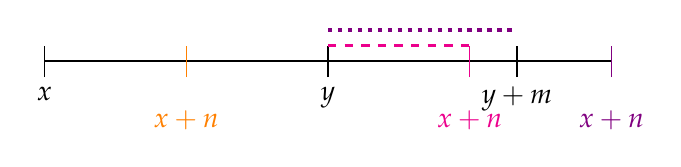
\begin{tikzpicture}[xscale=1.2]
	\draw [thick] (0,0) -- (6,0);

	\draw (0,-.2) -- (0, .2);
		\draw [orange] (1.5,-.2) -- (1.5, .2); % 1er cas
	\draw (3,-.2) -- (3, .2);
		\draw [magenta] (4.5,-.2) -- (4.5, .2); % 2ème cas
		\draw [-] [draw=magenta, dashed, very thick] (3,0.2) -- (4.5,0.2); % 2ème cas
	\draw (5,-.2) -- (5, .2);
		\draw [violet] (6,-.2) -- (6, .2); % 3ème cas
		\draw [-] [draw=violet, dotted, ultra thick] (3,0.4) -- (5,0.4); % 3ème cas
	
	\node[align=left, below] at (0,-.2)%
	{$x$};
	\node[align=left, below] at (3,-.2)%
	{$y$};
	\node[align=left, below] at (5,-.2)%
	{$y + m$};
	
	\node[align=left, below] at (1.5,-.5) %1er cas
	{\color{orange}{$x + n$}};
	\node[align=left, below] at (4.5,-.5) %2ème cas
	{\color{magenta}{$x + n$}};
	\node[align=left, below] at (6,-.5) %3ème cas
	{\color{violet}{$x + n$}};
\end{tikzpicture}

%\textbf{Raccourci} pour s'en souvenir où $\ell_a$ est le nombre inital de personnes :
%
%$\text{Cov}( \text{Groupe A}, \text{Groupe B} ) = $
%\begin{align*}
%	&\text{E}\{\text{être dans les groupes A et B}\} \\
%	&- \frac{\text{E}\{\text{être dans le groupe A}\} 
%	\times \text{E}\{\text{être dans le groupe B}\}}{\ell{a}} \Bigg]
%\end{align*}
Raccourci:
$\text{Cov}( \text{A}, \text{B} ) = \esp{A \cap B} - \frac{\esp{A}\esp{B}}{\ell{a}}$
%\subsubsection*{Lien entre $\ell_x$ et $S_X(x)$}
%
%\begin{align*}
%	\ell_x &= \ell_a S_{T_a}(x - a) = \ell_a \ \px[x - a]{a}
%\end{align*}


\section{Contrats d'assurance-vie}
%Le paiement est soit en continu, soit à la fin de l'année ou à la fin de la $\frac{1}{m}$ d'année.

\subsection{Notation et introduction}

\subsubsection*{Fonctions}

\begin{enumerate}
	\item[$a(T)$: ] Facteur d'accumulation.
	\item[$v(T)$: ] Facteur d'actualisation.
	\[
		v(t) = \frac{1}{a(t)}
	\]
	\item[$Z$ : ] v.a. de la valeur actualisée du montant payé selon les termes du contrat.
	\[
		Z = z_t = b(T) v(f(T))
	\]
	\item[$b(T)$: ] Prestation prévue en fonction de T.
	\item[$f(T)$: ] Montant du paiement en fonction de T. \\
	De plus, puisque $f(T)$ n'a pas d'importance lorsque $b(T) = 0$, on défini son domaine pour simplifier des interprétations plus tard.
	\[
		f(t) \ge T
	\]
	\item[$A$ : ] Pour simplifier la notation, on dénote la \textbf{prime unique nette \textit{(PUN)}} par :
	\begin{align*}
		\esp{Z} &= A_{x} = \int_{0}^{\omega - x} z_t \ \px[t]{x} \mu_{x + t} dt
	\end{align*}
	Le nom vient du fait qu'elle n'est payée qu'une seule fois \textit{(unique)} et qu'elle ne couvre que le coût des prestations \textit{(nette)}.
\end{enumerate}

\subsubsection*{Prestations}

\[
{{\color{cyan}{\boxed{}}}}\text{}^{{\color{gray}{\boxed{}}}}_{{\color{brown}{\boxed{}}}}\text{}_{{\color{blue}{\boxed{}}}}^{{\color{violet}{\boxed{}}}}\prescript{}{{\color{ao(english)}{\boxed{}}}}Ax_{{\color{red}{\boxed{}}}}^{{\color{magenta}{\boxed{}}}}
\]

\textbf{{\color{cyan}{\textbf{Prestation de base}}}}
\begin{itemize}
	\item[$b \Ax{x}$] Si quelque chose est payable c'est b.
	\item[$b \IA_x$] Paye b lorsqu'il y a décès à la \textbf{fin} de la \textit{première année} de couverture.
	\item[$b \DA_x$] Paye b lorsqu'il y a décès au \textbf{début} de la \textit{dernière année} de couverture.
\end{itemize}

\textbf{{\color{gray}{\textbf{Force, ou multiple j de la, d'intérêt $\delta$}}}}

$0 \leq \delta < 1 \text{ et } j \in \mathbb{Z}_+$
\begin{itemize}
	\item[$\prescript{\delta}{}{A}_x$] Évaluation avec \textbf{force} d'intérêt $\delta$ \textit{(constante)}.
	\item[$\prescript{j}{}{A}_x$] Évaluation avec \textbf{\textit{j} fois force} d'intérêt $\delta$ \textit{(pas nécessairement constante)}.
\end{itemize}

\textbf{\textcolor{brown}{Période différée}}
\begin{itemize}
	\item[$\prescript{}{m|}A_{x}$] Couverture débutant dans n années.\\
	\textbf{\textit{Donc}} si décède avant les m années, il n'y a pas de paiements.
\end{itemize}

\textbf{{\color{violet}{Fréquence de variation}}} \\
{\color{violet}{variation m fois par année}}
\begin{align*}
	\ImA_{x} \text{ et } \DmA_{x} 
\end{align*}
{\color{violet}{\textit{(dé)}croissance continue}}
\begin{align*}
	\IbA_x \text{ et } \DbA_x 
\end{align*}

\textbf{\textcolor{blue}{Type de variation de la prestation}}
\begin{itemize}
	\item[$A_{x}$] Constant
	\item[$\IA{x}$] Croissant arithmétiquement
	\item[$\DA{x}$] Décroissant arithmétiquement
\end{itemize}

\textbf{{\color{ao(english)}{\textbf{Durée temporaire de la variation}}}}\\
$\twoletsymb{I_{\angln}}{A}_{x}$ Augmentation uniquement lors des n premières années de couverture.

\textbf{{\color{magenta}{\textbf{Moment de paiement de la prestation de décès}}}}
\begin{itemize}
	\item[$\bar{A}_x$] Au moment du décès.
	\item[$\Ax{x}^{(m)}$] À la fin du 1/m année du décès.\\
	\textit{Pour exemple}, si $m = 12$ alors c'est payable à la fin du mois de décès.
\end{itemize}

\textbf{\textcolor{red}{Couverture temporaire n années}}
\begin{itemize}
	\item[$\Ax{\termxn}$] Cas de décès.
	\item[$\Ax{\pureendowxn}$] Cas de survie.
	\item[$\Ax{x:\angln}$] Les deux cas.
	\item[$\Ax{x}$] En tout temps.
\end{itemize}

\subsubsection*{Principes de calcul de la prime pour un seul contrat}


Principes pour calculer la prime \textit{(unique)} à payer pour un contrat d'assurance:
\begin{enumerate}
	\item $\esp{Z}$ \textbf{principe d'équivalence}
	\item $\esp{Z} + k \sigma_Z$
	\item $\xi$ \textbf{quantile de} $Z$.\\
\end{enumerate}

Interprétations pour un seul contrat
\begin{enumerate}
	\item En moyenne l'assureur ne fait ni gains ni pertes
	\item Lorsqu'il y a plusieurs contrats, le principe est équivalent au troisième mais lorsqu'il n'y en a qu'un seul alors il ne tient pas.
	\item Plus petite prime $\pi$ telle que $Pr(Z \ge \pi) = p$
\end{enumerate}

\subsubsection*{Principes de calcul pour un portefeuille de plusieurs contrats}

Généralement, on suppose les $n$ différents contrats $Z_{j}$ d'être identique et les vies à être indépendantes \textit{(i.i.d.)}.

\begin{align*}	
	S &= \sum_{j = 1}^{n} Z_j 
\end{align*}

\begin{enumerate}
	\item[1. ] Par le \textbf{principe d'équivalence}, $\esp{Z} = \pi$.
	\item[3. ] \textbf{Principe du quantile }$Pr(S \le n \pi) \ge p$, où $p$ est la \textbf{probabilité de solvabilité}.
\end{enumerate}

Cependant, si les contrats ne sont \textbf{\textit{pas identique}}, la \textbf{prime varie }selon le contrat.
\begin{enumerate}
	\item[1. ] Pour chaque type de contrat le \textbf{principe d'équivalence} ne change pas, $\esp{Z} = \pi$.
	\item[3. ] Pour le \textbf{Principe du quantile }on veut maintenant une \textbf{surchage égale} pour tous les contrats et donc le plus petite h telle que $Pr(S \le h) \ge p$.
	\item[$h$ : ] Prime collective sous le principe du quantile.
\end{enumerate}

Doit trouver la surchage $\theta$ qui, lorsqu'appliqué à chacune des espérances individuelles, donnera la prime collective au total.

\begin{enumerate}
	\item[$\theta$ : ] \textbf{Surchage}
\begin{align*}
		\pi &= (1 + \theta) \esp{Z} \\
		h &= (1 + \theta) \esp{S} 
\end{align*}
	\item[] \textbf{Suprime}
	\[
		\theta \esp{Z}
	\]
\end{enumerate}

Puisque par défaut les $Z_{j}$ sont \textit{(iid)} on applique \textbf{l'approximation normale} avec $S \sim N(\esp{S} = n \esp{Z}, V(S) = nV(Z))$.

%On peut alors obtenir le quantile de niveau $1 - \alpha$ de $S$ par le principe du quantile:

$\Phi^{-1}(p) = z_{1 - p}$

\begin{align*}
	z_{1 - p} &\le \frac{\sqrt{n} ( \pi - \esp{Z}}{\sigma_{Z}})\\
	\pi &\ge \esp{Z} + z_{1 - p} \left(\frac{\sigma_{Z}}{\sqrt{n}}\right) = \pi_p &
	\pi\$ &= \frac{\lceil 100 \pi_p \rceil}{100} \\
	n &\ge \left(\frac{z_{1 - p}\sigma_{Z}}{\pi - \esp{Z}}\right)^2 = n_{p} 
\end{align*} 

Donc avec $h$ on résoud $h = (1 + \theta) \esp{Z}$ et applique la surprime à tous les assurés.

%Si une même vie achète plusieurs contrats d'assurance vie, faut tenir compte des covariances.

\subsubsection*{Règle des moments}

%Lorsque $b_{t}^{j} = b_{t}, t \ge 0$, alias $b_{t} \in \{ 0, 1\}$, alors:
%\begin{align*}
%	\esp{Z^{j}}@\delta_{t} &= \esp{Z}@ j \times \delta_{t}
%\end{align*}
%Sinon on généralise:
\begin{align*}
	\esp{Z^{j}}@\delta_{t} &= \esp{b \times Z'^{j}}@\delta_{t} \\
	&= b^{j} \times \esp{Z'}@ j \times \delta_{t}
\end{align*}
Où $Z = bZ'$, donc $Z'$ est la v.a. équivalente avec une prestation unitaire.\\
À noter que la règle est \textbf{seulement applicable} aux \textbf{prestations nivelées} et donc n'est pas applicable aux prestations variants arithmétiquement.


\subsection{Payable au moment du décès}

Le \textit{montant} et \textit{moment du paiement} ne dépendent que du \textbf{temps écoulé depuis l'émission de la police}.\\
De plus, toutes nos fonctions sont définies en fonction de la v.a. de la durée de vie future de l'assuré $T$.

\subsubsection*{\textcolor{amber(sae/ece)}{Assurance à prestation nivelée}}

\paragraph{Assurance-vie entière} 

Est en vigueur tant que l'assuré est en vie et verse une prestation au moment de son décès.

\begin{align*}
\Ax*{x} 
	&= \int_{0}^{\omega - x} v^t \px[t]{x} \mu_{x+t} dt 
\end{align*}

\paragraph{Assurance-vie temporaire} Si l'assuré décède dans les $n$ années suivant l'émission du contrat, paye une prestation de décès.
\begin{align*}
\Ax*{\termxn}	
	&= \int_{0}^{n} v^t \px[t]{x} \mu_{x+t} dt 
\end{align*}

\paragraph{Capital différé de n années} Si l'assuré \textbf{\textit{ne décède pas}} dans les $n$ années suivant l'émission du contrat, paye une prestation de survie.\\
À noter qu'il est aussi connu comme le \textbf{facteur d'actualisation actuariel}.

\begin{align*}
	\Ax*{\pureendowxn}	
		&\Leftrightarrow \Ax{\pureendowxn}
		= v^{n} \px[n]{x} 
		= \Ex[m]{x}
\end{align*}

\paragraph{Assurance mixte} Si l'assuré \textbf{\textit{ne décède pas}} dans les $n$ annés suivant l'émission du contrat, paye une prestation de décès. S'il est toujours en vie, paye une prestation de survie.
\begin{align*}
\Ax*{x:\angln}	
	&= \int_{0}^{n} v^t \px[t]{x} \mu_{x+t} dt + v^n \px[n]{x} \\
	&= \Ax*{\termxn} + \Ax{\pureendowxn} 
\end{align*}

\paragraph{Assurance différée de m années} Si l'assuré décède \textbf{après} les $m$ année suivant l'émission du contrat, paye une prestation de décès.

\begin{align*}
\Ax*[m|]{x}	
	&= \int_{m}^{\omega -x} v^t \px[t]{x} \mu_{x+t} dt \\
	&= v^m \px[m]{x} \int_{0}^{\omega - x - m} v^s \px[s]{x+m} \ \mu_{(x+m)+s} \ ds \\
	&= v^m \px[m]{x} \Ax*{x+m} = \Ex[m]{x} \Ax*{x+m} 
\end{align*}

\paragraph{Lien entre assurance différée, assurance vie entière et assurance-vie temporaire}
\begin{align*}
\Ax*[m|]{x}		&= \Ax*{x} - \Ax*{\itop{x}:\angl{m}} \\
\end{align*}

\textbf{Comparaison des différents contrats}

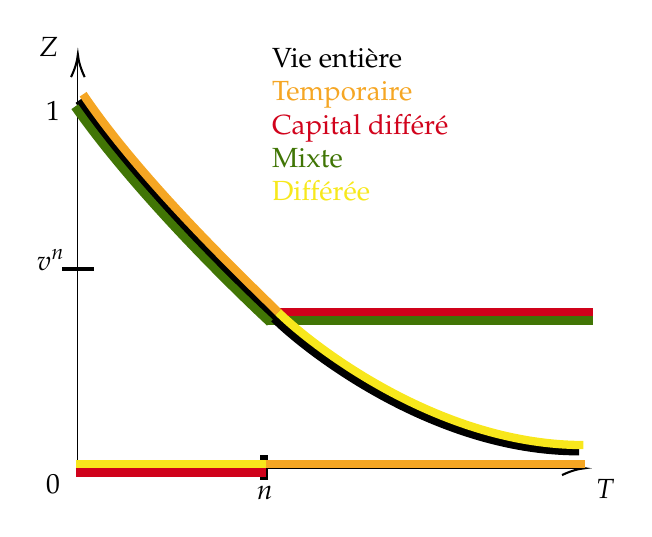
\begin{tikzpicture}[x=0.75pt,y=0.75pt,yscale=-1,xscale=1]
%uncomment if require: \path (0,300); %set diagram left start at 0, and has height of 300

%Straight Lines [id:da3016673697971952] 
\draw [color={rgb, 255:red, 208; green, 2; blue, 27 }  ,draw opacity=1 ][line width=3]    (137.5,150) -- (291.16,150) ;


%Straight Lines [id:da9102497979172233] 
\draw [color={rgb, 255:red, 65; green, 117; blue, 5 }  ,draw opacity=1 ][line width=3]    (134.5,154) -- (291.16,154) ;


%Curve Lines [id:da028008484781905985] 
\draw [line width=3]    (43.5,48) .. controls (72.5,91) and (123.5,139) .. (137.5,153) .. controls (151.5,167) and (213.5,217) .. (284.5,217) ;


%Curve Lines [id:da10931873289685323] 
\draw [color={rgb, 255:red, 248; green, 231; blue, 28 }  ,draw opacity=1 ][line width=3]    (139.5,150) .. controls (153.5,164) and (215.5,214) .. (286.5,214) ;


%Straight Lines [id:da5718298750755719] 
\draw    (42.96,225.18) -- (285.16,225.18) ;
\draw [shift={(287.16,225.18)}, rotate = 180] [color={rgb, 255:red, 0; green, 0; blue, 0 }  ][line width=0.75]    (10.93,-3.29) .. controls (6.95,-1.4) and (3.31,-0.3) .. (0,0) .. controls (3.31,0.3) and (6.95,1.4) .. (10.93,3.29)   ;

%Straight Lines [id:da3391294570889458] 
\draw    (42.96,225.18) -- (42.96,58.4) -- (42.96,27.8) ;
\draw [shift={(42.96,25.8)}, rotate = 450] [color={rgb, 255:red, 0; green, 0; blue, 0 }  ][line width=0.75]    (10.93,-3.29) .. controls (6.95,-1.4) and (3.31,-0.3) .. (0,0) .. controls (3.31,0.3) and (6.95,1.4) .. (10.93,3.29)   ;

%Straight Lines [id:da5827723542208845] 
\draw [line width=1.5]    (35.5,129) -- (50.5,129) ;


%Straight Lines [id:da9117414884275186] 
\draw [line width=3]    (132.5,219) -- (132.5,231) ;


%Straight Lines [id:da6911491942214352] 
\draw [color={rgb, 255:red, 208; green, 2; blue, 27 }  ,draw opacity=1 ][line width=3]    (41.96,227.18) -- (133.5,227.18) ;


%Straight Lines [id:da1824669182947345] 
\draw [color={rgb, 255:red, 248; green, 231; blue, 28 }  ,draw opacity=1 ][line width=3]    (41.96,223) -- (133.5,223) ;


%Straight Lines [id:da7751043797180222] 
\draw [color={rgb, 255:red, 245; green, 166; blue, 35 }  ,draw opacity=1 ][line width=3]    (133.5,223) -- (287.16,223) ;


%Curve Lines [id:da349665360780564] 
\draw [color={rgb, 255:red, 245; green, 166; blue, 35 }  ,draw opacity=1 ][line width=3]    (45.5,45) .. controls (74.5,88) and (125.5,136) .. (139.5,150) ;


%Curve Lines [id:da308588298202902] 
\draw [color={rgb, 255:red, 65; green, 117; blue, 5 }  ,draw opacity=1 ][line width=3]    (41.5,51) .. controls (72.5,95) and (121.5,142) .. (135.5,155) ;



% Text Node
\draw (297,235) node  [align=left] {$\displaystyle T$};
% Text Node
\draw (29,22) node  [align=left] {$\displaystyle Z$};
% Text Node
\draw (31,53) node  [align=left] {$\displaystyle 1$};
% Text Node
\draw (30,125) node  [align=left] {$\displaystyle v^{n}$};
% Text Node
\draw (133,237) node  [align=left] {$\displaystyle n$};
% Text Node
\draw (31,233) node  [align=left] {$\displaystyle 0$};
% Text Node
\draw (179,61) node  [align=left] {$\displaystyle  \begin{array}{{>{\displaystyle}l}}
\text{Vie entière}\\
\textcolor[rgb]{0.96,0.65,0.14}{\text{Temporaire}}\\
\textcolor[rgb]{0.82,0.01,0.11}{\text{Capital différé}}\\
\textcolor[rgb]{0.25,0.46,0.02}{\text{Mixte}}\\
\textcolor[rgb]{0.97,0.91,0.11}{\text{Différée}}
\end{array}$};


\end{tikzpicture}

%\textbf{Formule générale de la fonction de répartition}

%\begin{align*}
%	F_{\bar{Z}_x}(z) &= \left\{
%		\begin{matrix}
%			0	&	z < 0 \\
%			0	&	0 \le z < v^{\omega - x} \\
%			\px[-\frac{1}{\delta}ln(z)]{x}	&	v^{\omega - x}  \le z < 1 \\
%			1 	&	z \ge 1 \\
%		\end{matrix}	\right.
%\end{align*}

\subsubsection*{\textcolor{amber(sae/ece)}{Assurance à prestation variant arithmétiquement}}

\paragraph{Assurance Vie temporaire croissante} 

\begin{enumerate}
	\item[] Le capital \textbf{croit annuellement}.\\
	La prestation est de 1 \$ dans la première année, 2 \$ dans la deuxième, etc. jusqu'à n \$ dans la $n^{\text{ème}}$ année.

\begin{align*}
	\IA*_{\termxn}  &= \int_0^n (1 + \lfloor t \rfloor) v^t \px[t]{x} \mu_{x+t} dt \\
		&= \actsymb{\bar{A}}{\nthtop{1}{x}:\angln} + \actsymb[1|]{\bar{A}}{\nthtop{1}{x}:\angl{n-1}} + ... + \actsymb[n-1|]{\bar{A}}{\nthtop{1}{x}:\angl1}
\end{align*}

\end{enumerate}

\tikzset{every picture/.style={line width=0.75pt}} %set default line width to 0.75pt        

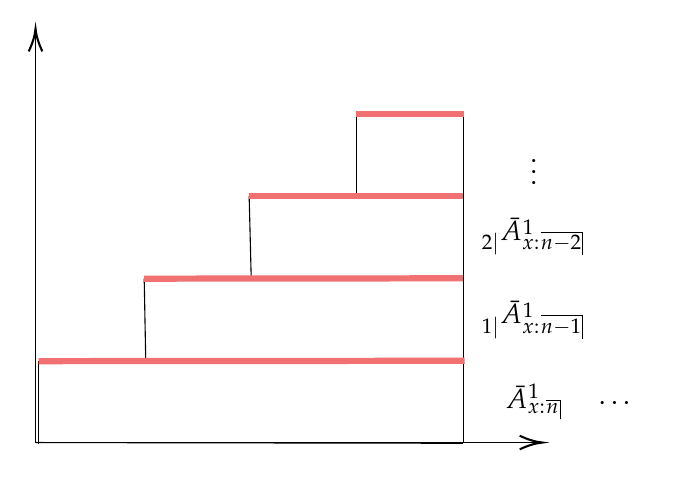
\begin{tikzpicture}[x=0.75pt,y=0.75pt,yscale=-1,xscale=1]
%uncomment if require: \path (0,460.60000228881836); %set diagram left start at 0, and has height of 460.60000228881836

%Shape: Rectangle [id:dp2153664891645204] 
\draw  [draw opacity=0][fill={rgb, 255:red, 255; green, 255; blue, 255 }  ,fill opacity=1 ] (63.06,164.97) -- (11.5,164.97) -- (11.5,204.7) -- (63.06,204.7) -- cycle ;
%Shape: Rectangle [id:dp5225981801630806] 
\draw  [draw opacity=0][fill={rgb, 255:red, 255; green, 255; blue, 255 }  ,fill opacity=1 ] (164.44,85.49) -- (112.88,85.49) -- (112.88,204.36) -- (164.44,204.36) -- cycle ;
%Shape: Rectangle [id:dp5069530248534422] 
\draw  [draw opacity=0][fill={rgb, 255:red, 255; green, 255; blue, 255 }  ,fill opacity=1 ] (113.88,125.23) -- (62.32,125.23) -- (62.32,204.36) -- (113.88,204.36) -- cycle ;
%Shape: Rectangle [id:dp27824679166313815] 
\draw  [draw opacity=0][fill={rgb, 255:red, 255; green, 255; blue, 255 }  ,fill opacity=1 ] (216,45.75) -- (164.44,45.75) -- (164.44,204.36) -- (216,204.36) -- cycle ;
%Straight Lines [id:da936615963108024] 
\draw    (9.96,204.18) -- (252.16,204.18) ;
\draw [shift={(254.16,204.18)}, rotate = 180] [color={rgb, 255:red, 0; green, 0; blue, 0 }  ][line width=0.75]    (10.93,-3.29) .. controls (6.95,-1.4) and (3.31,-0.3) .. (0,0) .. controls (3.31,0.3) and (6.95,1.4) .. (10.93,3.29)   ;

%Straight Lines [id:da09653378675557245] 
\draw    (216,204.36) -- (216,45.75) ;


%Straight Lines [id:da46946353778662164] 
\draw    (9.96,204.18) -- (215.81,204.53) ;


%Straight Lines [id:da2160350807468463] 
\draw    (63.06,164.97) -- (62.32,125.23) ;


%Straight Lines [id:da2909730871778471] 
\draw    (11.5,204.7) -- (11.5,164.97) ;


%Straight Lines [id:da9752575748839756] 
\draw    (113.88,125.23) -- (112.88,85.49) ;


%Straight Lines [id:da2098155502707164] 
\draw    (164.44,85.49) -- (164.44,45.75) ;


%Straight Lines [id:da5631700682235457] 
\draw [color={rgb, 255:red, 241; green, 112; blue, 113 }  ,draw opacity=1 ][line width=2.25]    (216.34,45.75) -- (164.44,45.75) ;
%Straight Lines [id:da28001017635075276] 
\draw [color={rgb, 255:red, 241; green, 112; blue, 113 }  ,draw opacity=1 ][line width=2.25]    (112.88,85.49) -- (216,85.49) ;
%Straight Lines [id:da30632392932152186] 
\draw [color={rgb, 255:red, 241; green, 112; blue, 113 }  ,draw opacity=1 ][line width=2.25]    (62.32,125.23) -- (216,125.05) ;
%Straight Lines [id:da7928314458046128] 
\draw [color={rgb, 255:red, 241; green, 112; blue, 113 }  ,draw opacity=1 ][line width=2.25]    (11.5,164.97) -- (216.75,164.79) ;
%Straight Lines [id:da5692973763116236] 
\draw    (9.96,204.18) -- (9.96,6.8) ;
\draw [shift={(9.96,4.8)}, rotate = 450] [color={rgb, 255:red, 0; green, 0; blue, 0 }  ][line width=0.75]    (10.93,-3.29) .. controls (6.95,-1.4) and (3.31,-0.3) .. (0,0) .. controls (3.31,0.3) and (6.95,1.4) .. (10.93,3.29)   ;


% Text Node
\draw (290,185) node  [align=left] {$\dots$};
\draw (250,185) node  [align=left] {$\actsymb{\bar{A}}{\nthtop{1}{x}:\angln}$};
\draw (250,145) node  [align=left] {$\actsymb[1|]{\bar{A}}{\nthtop{1}{x}:\angl{n-1}}$};
\draw (250,105) node  [align=left] {$\actsymb[2|]{\bar{A}}{\nthtop{1}{x}:\angl{n-2}}$};
\draw (250,70) node  [align=left] {$\vdots$};
\end{tikzpicture}

\begin{enumerate}

	\item[] Le capital \textbf{croît \textit{(annuellement)} pendant r années}.\\
\begin{align*}
	\twoletsymb{I_{\anglr}}{\bar{A}}_{\termxn} 
		&= \sum_{k = 0}^{r - 1} \Ax*[k|]{\nthtop{1}{x}:\angl{n-k}} 
%	\\ 	&= \IA*_{\termxn} + r \Ax*[r|]{\nthtop{1}{x}:\angl{n-r}}
\end{align*}

	\item[] Le capital \textbf{croît m fois par année}.\\
	Paye une prestation de 1/m \$ dans le premier 1/m d'année, 2/m \$ dans le deuxième, etc.

\begin{align*}
	\twoletsymb{I^{(m)}}{\bar{A}}_{\nthtop{1}{x}:\angln} 
	&= \int_0^n \frac{([t \times m] + 1)}{m} v^t \px[t]{x} \mu_{x+t} dt 
\end{align*}


	\item[] Le capital est \textbf{différé de r années}.

\begin{align*}
	\prescript{}{r|}{\IA*_{\termxn}} 
	&= v^{r}\px[r]{x}\IA*_{\nthtop{1}{x} + r:\angln}
\end{align*}

	\item[] Le capital \textbf{croît continûment}.\\
	Paye une prestation de t au moment du décès, tant qu'il se produise dans les n premières années.

\begin{align*}
	\IbA*_{\termxn} 
	&=  \int_0^n t v^t \px[t]{x} \mu_{x+t} dt \\
	&= 	\int_0^n \prescript{}{s|}{\bar{A}_{\nthtop{1}{x}:\angl{n-s}}} ds
\end{align*}

\end{enumerate}

\paragraph{Assurance Vie temporaire décroissante} 


\begin{enumerate}

	\item[] Le capital \textbf{décroit chaque année} et donc la prestation doit nécessairement être une temporaire.\\
	Paye n \$ au début de la première année, n-1 \$ au début de la deuxième, etc. jusqu'à 1 \$ au début de la dernière année.\\
	On peut le voir de l'autre sens, la prestation du début de la dernière année est de 1 \$, 2 \$ au début de l'avant dernière année, etc. 
	
\begin{align*}
	\DA*_{\termxn}  &= \int_0^{\omega - x} (n - \lfloor t \rfloor) v^t \px[t]{x} \mu_{x+t} dt \\
		&= \actsymb{\bar{A}}{\nthtop{1}{x}:\angl1} + \actsymb{\bar{A}}{\nthtop{1}{x}:\angl2} + ... + \actsymb{\bar{A}}{\nthtop{1}{x}:\angln}
\end{align*}

\end{enumerate}

\tikzset{every picture/.style={line width=0.75pt}} %set default line width to 0.75pt        

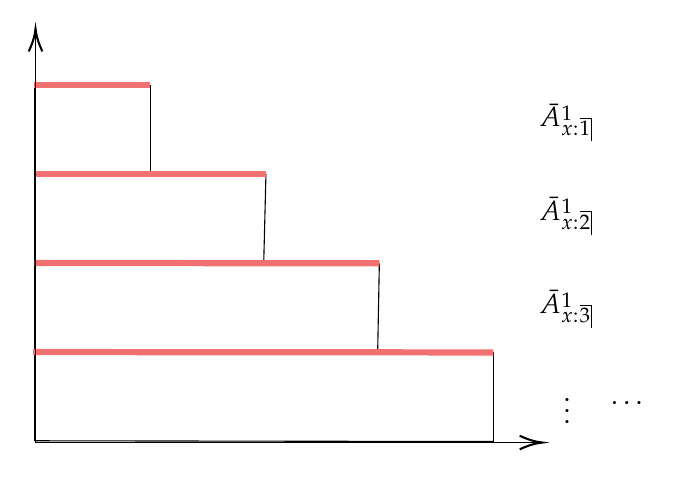
\begin{tikzpicture}[x=0.75pt,y=0.75pt,yscale=-1,xscale=1]
%uncomment if require: \path (0,300); %set diagram left start at 0, and has height of 300

%Shape: Rectangle [id:dp8249508548173892] 
\draw  [draw opacity=0][fill={rgb, 255:red, 255; green, 255; blue, 255 }  ,fill opacity=1 ] (218.79,225.77) -- (274.5,225.77) -- (274.5,268.7) -- (218.79,268.7) -- cycle ;
%Shape: Rectangle [id:dp288679577114328] 
\draw  [draw opacity=0][fill={rgb, 255:red, 255; green, 255; blue, 255 }  ,fill opacity=1 ] (109.26,139.9) -- (164.97,139.9) -- (164.97,268.33) -- (109.26,268.33) -- cycle ;
%Shape: Rectangle [id:dp44620071768330805] 
\draw  [draw opacity=0][fill={rgb, 255:red, 255; green, 255; blue, 255 }  ,fill opacity=1 ] (163.89,182.84) -- (219.6,182.84) -- (219.6,268.33) -- (163.89,268.33) -- cycle ;
%Shape: Rectangle [id:dp6514753834850957] 
\draw  [draw opacity=0][fill={rgb, 255:red, 255; green, 255; blue, 255 }  ,fill opacity=1 ] (53.55,96.97) -- (109.26,96.97) -- (109.26,268.33) -- (53.55,268.33) -- cycle ;
%Straight Lines [id:da9129710482760682] 
\draw    (53.96,269.18) -- (296.16,269.18) ;
\draw [shift={(298.16,269.18)}, rotate = 180] [color={rgb, 255:red, 0; green, 0; blue, 0 }  ][line width=0.75]    (10.93,-3.29) .. controls (6.95,-1.4) and (3.31,-0.3) .. (0,0) .. controls (3.31,0.3) and (6.95,1.4) .. (10.93,3.29)   ;

%Straight Lines [id:da14257233357209076] 
\draw    (53.55,268.33) -- (53.55,96.97) ;


%Straight Lines [id:da638927749516857] 
\draw    (53.55,268.33) -- (274.5,268.7) ;


%Straight Lines [id:da863275927987611] 
\draw    (218.79,225.77) -- (219.6,182.84) ;


%Straight Lines [id:da3684296762771002] 
\draw    (274.5,268.7) -- (274.5,225.77) ;


%Straight Lines [id:da15964539835120828] 
\draw    (163.89,182.84) -- (164.97,139.9) ;


%Straight Lines [id:da7596730836489285] 
\draw    (109.26,139.9) -- (109.26,96.97) ;


%Straight Lines [id:da601078444755968] 
\draw [color={rgb, 255:red, 241; green, 112; blue, 113 }  ,draw opacity=1 ][line width=2.25]    (53.19,96.97) -- (109.26,96.97) ;


%Straight Lines [id:da9731248181909757] 
\draw [color={rgb, 255:red, 241; green, 112; blue, 113 }  ,draw opacity=1 ][line width=2.25]    (164.97,139.9) -- (53.55,139.9) ;


%Straight Lines [id:da863495199913406] 
\draw [color={rgb, 255:red, 241; green, 112; blue, 113 }  ,draw opacity=1 ][line width=2.25]    (219.6,182.84) -- (53.55,182.65) ;


%Straight Lines [id:da5633099918008455] 
\draw [color={rgb, 255:red, 241; green, 112; blue, 113 }  ,draw opacity=1 ][line width=2.25]    (274.5,225.77) -- (52.75,225.58) ;


%Straight Lines [id:da9424905462587518] 
\draw    (53.96,269.18) -- (53.96,102.4) -- (53.96,71.8) ;
\draw [shift={(53.96,69.8)}, rotate = 450] [color={rgb, 255:red, 0; green, 0; blue, 0 }  ][line width=0.75]    (10.93,-3.29) .. controls (6.95,-1.4) and (3.31,-0.3) .. (0,0) .. controls (3.31,0.3) and (6.95,1.4) .. (10.93,3.29)   ;


% Text Node
\draw (340,250) node  [align=left] {$\dots$};
\draw (310,250) node  [align=left] {$\vdots$};
\draw (310,205) node  [align=left] {$\bar{A}_{\nthtop{1}{x}:\angl{3}}$};
\draw (310,160) node  [align=left] {$\bar{A}_{\nthtop{1}{x}:\angl{2}}$};
\draw (310,115) node  [align=left] {$\bar{A}_{\nthtop{1}{x}:\angl{1}}$};

\end{tikzpicture}



\begin{enumerate}

	\item[] Le capital \textbf{décroît m fois par année}.\\
	Paye une prestation de n \$ dans le premier 1/m d'année, n - 1/m \$ dans le deuxième, etc. jusqu'à 1/m \$ durant le dernier 1/m d'année.

\begin{align*}
	\twoletsymb{D^{(m)}}{\bar{A}}_{\nthtop{1}{x}:\angln} &= \int_0^n \left(n - \frac{1}{m} \times [m t] \right) v^t \px[t]{x} \mu_{x+t} dt 
\end{align*}

	\item[] Le capital est \textbf{différé de r années}.

\begin{align*}
	\prescript{}{r|}{\DA*_{\termxn}} 
	&= \sum_{k = 1}^{n} \Ax[r|]{\nthtop{1}{x}:\angl{k}} 
%	\\ &= v^{r}\px[r]{x}\DA*_{\nthtop{1}{x} + r:\angln}\\
\end{align*}

	\item[] Le capital \textbf{décroît continûment}.\\
	Prévoit une prestation de n \$ pour un décès immédiat, par la suite la prestation décroît linéairement jusquà 0 \$ au bout de n années.

\begin{align*}
	\DbA*_{\termxn} &= \int_0^{n} (n - t) v^t \px[t]{x} \mu_{x+t} dt \\
	&= \int_0^{n} \bar{A}_{\nthtop{1}{x:}{\angl{s}}} ds
\end{align*}

\end{enumerate}

\paragraph{Assurance mixte}

\begin{enumerate}
	\item[] L'assurance peut être mixte peut importe qu'elle soit croissante ou décroissante.
	\item[] L'assurance \textit{\textbf{croissante}} mixte n années, paierait n\$ en cas de survie \textit{(peu importe la fréquence de la croissance)}.
	\begin{align*}
		\IA*_{x:\angln} &= \IA*_{\nthtop{1}{x}:\angln}  + n {\prescript{}{n}E_{x}} 
	\end{align*}
	\item[] L'assurance \textit{\textbf{décroissante}} mixte n années, paierait 1/m\$ en cas de survie si la prestation \textbf{décroît $m$ fois par année}.
	\item[] L'assurance \textit{\textbf{décroissante}} mixte n années, paierait 1\$ en cas de survie si la prestation \textbf{décroît à chaque année} \textit{(alias, m = 1)}.
	\item[] L'assurance \textit{\textbf{décroissante}} mixte n années aurait une prestation de survie nulle si la prestation \textbf{décroît continûment}. Donc, en théorie une assurance décroissant continûment peut être mixte mais pas en pratique.
	\item[] Comme pour les assurances à prestations constantes, une mixte est la combinaison d'une temporaire \textit{(avec la même (dé)croissance)} et d'un capital différé.
\end{enumerate}

\begin{align*}
	\prescript{}{r|}{\DA*_{x:\angln}} &= \prescript{}{r|}{\DA*_{\termxn}} + \Ax{x:\nthtop{1}{\angl{n + r}}}
\end{align*}

\paragraph{Assurance Vie entière croissante}

\begin{enumerate}

\item[] Le capital \textbf{croît chaque année}. \\
La formule est équivalente à remplacer $n$ par $\omega - x$ dans les formules de l'assurance vie temporaire $n$ années.\\ 
Donc, 1 \$ la première, 2 \$ la deuxième, etc. jusqu'à \textbf{$\omega - x$}\$ la dernière.

\begin{align*}
	\IA*_{x} &= \int_0^{\omega - x} (1 + \lfloor t \rfloor) v^t \px[t]{x} \mu_{x+t} dt \\
		&= \Ax*{x} + \Ax*[1|]{x} + \Ax*[2|]{x} + ...
\end{align*}

\item[] Le capital \textbf{croît continûment}. \\
La formule est équivalente à remplacer $n$ par $\omega - x$ dans les formules de l'assurance vie temporaire $n$ années.

\begin{align*}
	\IbA*_x &= \int_0^{\omega - x} t v^t \px[t]{x} \mu_{x+t} dt \\
		&= \int_0^{\omega - x} \Ax*[s|]{x} ds 
\end{align*}

\item[] Le capital \textbf{croit \textit{(annuellement)} pendant $n$ années}.\\
Comme une vie entière sauf que la capital cesse de croître après n années et paye n\$ pour la suite.

\begin{align*}
	\twoletsymb{I_{\angl{n}}}{\bar{A}}_{x} 
%	&= \int_0^n (1 +  [t]) v^t \px[t]{x} \mu_{x+t} dt \\
%	& + \int_n^{\omega - x} n v^t \px[t]{x} \mu_{x+t} dt \\
	&= \IA*_{\termxn} + n \Ax*[n|]{x}\\
	&= \Ax*{x} + \Ax*[1|]{x} + ... + \Ax*[n-1|]{x}
%	\\ &= \Ax*{\nthtop{1}{x}:\angl{1}} + 2 \times \Ax*[1|]{\nthtop{1}{x}:\angl{1}} + 3 \times \Ax*[2|]{\nthtop{1}{x}:\angl{1}} + ... + n \times \Ax*[n-1|]{x}
\end{align*}

\end{enumerate}


\paragraph{Relations} 

\begin{align*}
%	\IA*_{\termxn} &= \IA*_{\nthtop{1}{x}:\angl{1}}  + {\prescript{}{1}E_{x}} \left[ \IA*_{\nthtop{1}{x + 1}:\angl{n - 1}} + \bar{A}_{\nthtop{1}{x + 1}:\angl{n - 1}}\right]\\
\twoletsymb{I_{\anglr}}{\bar{A}}_{\termxn} &= \IA*_{\nthtop{1}{x}:\anglr} + r \Ax*[r|]{\nthtop{1}{x}:\angl{n-r}}\\
	{\prescript{}{\color{teal}{r|}}{\IA*_{\termxn}}} &= v^{r} \px[r]{x} {\IA*_{\nthtop{1}{x + r}:\angln}}\\
	{\prescript{}{\color{teal}{r|}}{\DA*_{\termxn}}} &= v^{r}\px[r]{x}\DA*_{\nthtop{1}{x} + r:\angln}\\
\end{align*}
\begin{align*}
	{(D^{\color{red}{(m)}}\bar{A})_{\termxn}} + (I^{\color{red}{(m)}}\bar{A})_{\termxn} &= \left(n + \frac{1}{{\color{red}{(m)}}} \right) \bar{A}_{\termxn}\\
	{\prescript{}{\color{teal}{r|}}{\DbA*_{\termxn}}} + \prescript{}{\color{teal}{r|}}{\IbA*_{\termxn}}  &= n \Ax*[\color{teal}{r|}]{\termxn}\\	
	\DA*_{\nthtop{1}{x}:\angl{n-1}} + \twoletsymb{I_{\angln}}{\bar{A}}_{\nthtop{1}{x}} &= n \Ax*{\termxn}\\		
%	{\prescript{}{\color{teal}{r|}}{\DA*_{\termxn}}} + \prescript{}{\color{teal}{r|}}{\IA*_{\termxn}}  &= (n + 1) \Ax[\color{teal}{r|}]{\termxn}\\	
	{\prescript{}{\color{teal}{r|}}{\DA*_{\nthtop{1}{x}:\angl{n-1}}}} + \prescript{}{\color{teal}{r|}}{\IA*_{\termxn}}  &= n \Ax[\color{teal}{r|}]{\termxn}\\	
\end{align*}

\textbf{Relations croissance}
\begin{align*}
	\IbA*_{\termxn} &= {\color{blue_rectangle}{\IbA*_{\nthtop{1}{x}:\angl{1}}}} + v \px{x} \left[ {\color{green_rectangle}{\bar{A}_{\nthtop{1}{x + 1}:\angl{n - 1}}}} + {\color{red_rectangle}{\IbA*_{\nthtop{1}{x + 1}:\angl{n - 1}}}} \right]
\end{align*}

\tikzset{every picture/.style={line width=0.75pt}} %set default line width to 0.75pt        

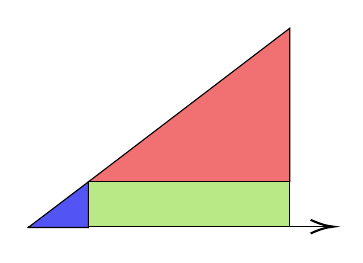
\begin{tikzpicture}[x=0.75pt,y=0.75pt,yscale=-1,xscale=1]
%uncomment if require: \path (0,300); %set diagram left start at 0, and has height of 300

%Straight Lines [id:da8341103379765638] 
\draw    (56.7,202) -- (201.7,202) ;
\draw [shift={(203.7,202)}, rotate = 180] [color={rgb, 255:red, 0; green, 0; blue, 0 }  ][line width=0.75]    (10.93,-3.29) .. controls (6.95,-1.4) and (3.31,-0.3) .. (0,0) .. controls (3.31,0.3) and (6.95,1.4) .. (10.93,3.29)   ;

%Straight Lines [id:da6472587459774688] 
\draw    (85.7,180.4) -- (85.7,202.4) ;


%Straight Lines [id:da6574015464366993] 
\draw    (85.7,180.4) -- (182.7,180.4) ;

%Shape: Right Triangle [id:dp954195254557896] 
\draw  [fill={rgb, 255:red, 241; green, 112; blue, 113 }  ,fill opacity=1 ] (182.7,106.4) -- (85.7,180.4) -- (182.7,180.4) -- cycle ;
%Shape: Right Triangle [id:dp6083621732280395] 
\draw  [fill={rgb, 255:red, 83; green, 84; blue, 244 }  ,fill opacity=1 ] (85.7,180.4) -- (56.7,202.4) -- (85.7,202.4) -- cycle ;
%Shape: Rectangle [id:dp08630244909166351] 
\draw  [fill={rgb, 255:red, 184; green, 233; blue, 134 }  ,fill opacity=1 ] (85.7,202) -- (182.7,202) -- (182.7,180.4) -- (85.7,180.4) -- cycle ;

\end{tikzpicture}

\textbf{Relations décroissance}
\begin{align*}
	\DbA*_{\termxn} &= {\color{green_rectangle}{(n - 1) \bar{A}_{\nthtop{1}{x}:\angl{1}}}} + {\color{blue_rectangle}{\DbA*_{\nthtop{1}{x}:\angl{1}}}} + v \px{x} {\color{red_rectangle}{\DbA*_{\nthtop{1}{x + 1}:\angl{n - 1}}}}
\end{align*}

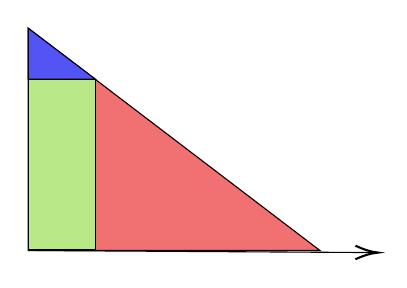
\begin{tikzpicture}[x=0.75pt,y=0.75pt,yscale=-1,xscale=1]
%uncomment if require: \path (0,300); %set diagram left start at 0, and has height of 300

%Straight Lines [id:da8341103379765638] 
\draw    (131.7,202.4) -- (294.7,203.39) ;
\draw [shift={(296.7,203.4)}, rotate = 180.35] [color={rgb, 255:red, 0; green, 0; blue, 0 }  ][line width=0.75]    (10.93,-3.29) .. controls (6.95,-1.4) and (3.31,-0.3) .. (0,0) .. controls (3.31,0.3) and (6.95,1.4) .. (10.93,3.29)   ;

%Straight Lines [id:da6472587459774688] 
\draw    (236.35,177.86) -- (236.35,202.4) ;


%Straight Lines [id:da6574015464366993] 
\draw    (236.35,177.86) -- (128.13,177.86) ;


%Shape: Right Triangle [id:dp954195254557896] 
\draw  [fill={rgb, 255:red, 241; green, 112; blue, 113 }  ,fill opacity=1 ] (128.13,95.3) -- (268.7,202.4) -- (128.13,202.4) -- cycle ;
%Shape: Right Triangle [id:dp6083621732280395] 
\draw  [fill={rgb, 255:red, 83; green, 84; blue, 244 }  ,fill opacity=1 ] (128.13,95.3) -- (160.48,119.84) -- (128.13,119.84) -- cycle ;
%Shape: Rectangle [id:dp08630244909166351] 
\draw  [fill={rgb, 255:red, 184; green, 233; blue, 134 }  ,fill opacity=1 ] (160.48,201.95) -- (128.13,201.95) -- (128.13,119.84) -- (160.48,119.84) -- cycle ;

\end{tikzpicture}
    
\begin{align*}
	\DA*_{\termxn} &= {\color{blue_rectangle}{n \bar{A}_{\nthtop{1}{x}:\angl{1}}}} + v \px{x} {\color{red_rectangle}{\DA*_{\nthtop{1}{x + 1}:\angl{n - 1}}}}
\end{align*}

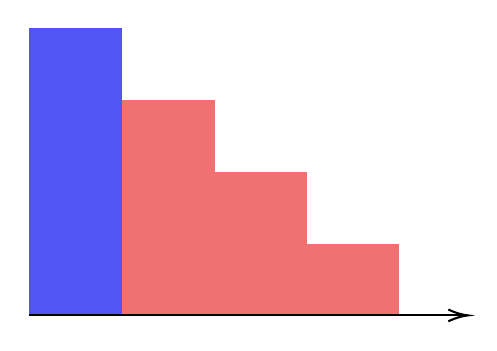
\begin{tikzpicture}[x=0.65pt,y=0.65pt,yscale=-1,xscale=1]
%uncomment if require: \path (0,300); %set diagram left start at 0, and has height of 300

%Shape: Rectangle [id:dp440986871106801] 
\draw  [draw opacity=0][fill={rgb, 255:red, 241; green, 112; blue, 113 }  ,fill opacity=1 ] (482.45,160.75) -- (534.35,160.75) -- (534.35,200.75) -- (482.45,200.75) -- cycle ;
%Shape: Rectangle [id:dp8956168288472683] 
\draw  [draw opacity=0][fill={rgb, 255:red, 241; green, 112; blue, 113 }  ,fill opacity=1 ] (380.4,80.75) -- (432.3,80.75) -- (432.3,200.4) -- (380.4,200.4) -- cycle ;
%Shape: Rectangle [id:dp8909221598764323] 
\draw  [draw opacity=0][fill={rgb, 255:red, 241; green, 112; blue, 113 }  ,fill opacity=1 ] (431.3,120.75) -- (483.2,120.75) -- (483.2,200.4) -- (431.3,200.4) -- cycle ;
%Shape: Rectangle [id:dp3313819257578299] 
\draw  [draw opacity=0][fill={rgb, 255:red, 83; green, 84; blue, 244 }  ,fill opacity=1 ] (328.5,40.75) -- (380.4,40.75) -- (380.4,200.4) -- (328.5,200.4) -- cycle ;
%Straight Lines [id:da8863050344236503] 
\draw [line width=0.75]    (328.5,200.4) -- (570.7,200.4) ;
\draw [shift={(572.7,200.4)}, rotate = 180] [color={rgb, 255:red, 0; green, 0; blue, 0 }  ][line width=0.75]    (10.93,-3.29) .. controls (6.95,-1.4) and (3.31,-0.3) .. (0,0) .. controls (3.31,0.3) and (6.95,1.4) .. (10.93,3.29)   ;
\end{tikzpicture}


\subsubsection*{\textcolor{amber(sae/ece)}{Assurance à prestation variant exponentiellement}}

La prestation de référence est celle payable en cas de décès immédiat.
La prestation est \textbf{\textit{indexée}} continûment à force $\tau$; généralement, $\tau < \delta$ et peut même être négatif.\\
Exemple pour une assurance temporaire n année différée de r années $\prescript{}{r|}{\bar{A}}_{\termxn}^{\;\; \text{ind}}$.\\
\begin{align*}
	Z &= \prescript{\delta - \tau}{r|}{\bar{Z}}_{\termxn}\\
	Z &= \left\{
	\begin{matrix}
		0	&	T < r \\
		e^{-(\delta - \tau) T}	&	r < T < r + n \\
		0	&	T > n + r
	\end{matrix}
	\right.
\end{align*}

\subsubsection*{\textcolor{amber(sae/ece)}{Évolution du fonds}}

\begin{enumerate}
\item[] Fonds initialement constitué des primes reçues pour $n$ contrats.
\begin{align*}
	F_{0} &= n \pi
\end{align*}
\item[\textbf{Augmente}] \textit{(croit)} avec le taux de rendement réalisé sur les placements.
\item[\textbf{Diminue}] \textit{(décroit)} chaque fois qu'une prestation est payable.
\item[$F_{t}$] : valeur du fonds à $t$ \textit{(après le paiement de prestations payables au temps t s'il y a lieu)}.
\end{enumerate}

Soit $t_1 < t_2 < \dots < t_n$ les \textbf{moments de décès} \textit{(en ordre croissant)}. 

Soit $\delta_s, \ s > 0$ la force d'intérêt réalisée à $s$.

Tant que des prestations de décès sont payables:
%\begin{align*}
%	F_{t_1^{-}} &= F_{0} \; e^{\int_0^{t_1} \delta_s ds} \\
%	F_{t_1^{+}} &= F_{t_1^{-}} - b(t_1)
%\end{align*}
\begin{align*}
	F_{t_j^{-}} &= F_{t_{j-1}^{+}} \; e^{\int_{t_{j-1}}^{t_j} \delta_s ds} \\
	F_{t_j^{+}} &= F_{t_j^{-}} - b(t_j)
\end{align*}

Si le contrat se termine à $r$ 
\begin{enumerate}
	\item[\textbf{sans}] prestation de survie.
	\begin{align*}
	F_{r} &= F_{t_{k}^{+}} \; e^{\int_{t_{k}}^{r} \delta_s ds} \\
	\text{où } t_k &= \max \{t_j | t_j < r\} 
	\end{align*}
	\item[\textbf{avec}] prestation de survie
	\begin{align*}
	F_{r} &= F_{t_{k}^{+}} \; e^{\int_{t_{k}}^{r} \delta_s ds} - b^{\star}(r)(n - k) \\
	\text{où } t_k &= \max \{t_j | t_j < r\}  \\
	\text{et } b^{\star}(r) &= \text{prestation de survie}  
	\end{align*}
\end{enumerate}

\subsection{Payable à la fin de l'année du décès}

La prestation peut seulement changer aux anniversaires de la police (alias aux âges entiers).

%Plus facile à calculer et donc souvent on va calculer la prestation payable à la fin de l'année et utiliser une relation pour établir la prime d'une assurance avec prestation payable au moment du décès.

L'information est souvent disponible sous format de table et donc les seuls calculs possible sont ceux des contrats payable à la fin de l'année du décès.

De façon générale, l'âge à l'émission, la durée de couverture et la période différée sont entiers $x, n, r \in \mathds{Z}$.

\subsubsection*{\textcolor{amber(sae/ece)}{Principe général}}

\begin{description}
	\item[Valeur actualisée :] $z_{k + 1}$
	\item[Prestation :] $b_{k + 1}$
	\item[Facteur d'actualisation :] $v_{k + 1}$
	\item[] $f(T) = [T + 1]$
\end{description}
$\forall K \in \mathds{Z}_+$ alias $(0, 1, 2, \dots)$
\begin{align*}
	Z 		&= z_{K + 1} = b_{K + 1} v_{K + 1} \\
	\esp{Z} &= \sum_{k = 0}^{\omega - x - 1} z_{k + 1} \, \qx[k|]{x}
\end{align*}

\textbf{Principe du quantile}: si on atteint entre 2 marches, on choisit toujours \textbf{\textit{la plus basse}}.

\begin{align*}
	\text{si } &t^{*} \not\in Z_{+}, \pi = Z|_{k = [t^{*}]} \\
	\text{si } &t^{*} \in Z_{+}, \pi = \text{min}(Z|_{k = t^{*}}, Z|_{k = t^{*}-1})
\end{align*}

\tikzset{every picture/.style={line width=0.75pt}} %set default line width to 0.75pt        

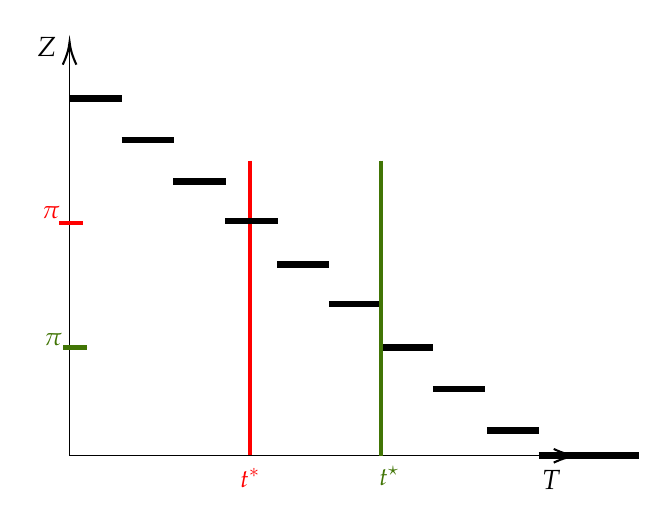
\begin{tikzpicture}[x=0.75pt,y=0.75pt,yscale=-1,xscale=1]
%uncomment if require: \path (0,300); %set diagram left start at 0, and has height of 300

%Straight Lines [id:da05705122517826289] 
\draw [color={rgb, 255:red, 255; green, 0; blue, 0 }  ,draw opacity=1 ][fill={rgb, 255:red, 255; green, 0; blue, 0 }  ,fill opacity=1 ][line width=1.5]    (122,69) -- (122,211.33) ;


%Straight Lines [id:da7157253876257526] 
\draw    (34.96,211.18) -- (277.16,211.18) ;
\draw [shift={(279.16,211.18)}, rotate = 180] [color={rgb, 255:red, 0; green, 0; blue, 0 }  ][line width=0.75]    (10.93,-3.29) .. controls (6.95,-1.4) and (3.31,-0.3) .. (0,0) .. controls (3.31,0.3) and (6.95,1.4) .. (10.93,3.29)   ;

%Straight Lines [id:da43893305379603675] 
\draw    (34.96,211.18) -- (34.96,13.8) ;
\draw [shift={(34.96,11.8)}, rotate = 450] [color={rgb, 255:red, 0; green, 0; blue, 0 }  ][line width=0.75]    (10.93,-3.29) .. controls (6.95,-1.4) and (3.31,-0.3) .. (0,0) .. controls (3.31,0.3) and (6.95,1.4) .. (10.93,3.29)   ;

%Straight Lines [id:da6053082774961389] 
\draw [line width=2.25]    (35,39) -- (60.17,39) ;


%Straight Lines [id:da3266616172184664] 
\draw [line width=2.25]    (60,59) -- (85.17,59) ;


%Straight Lines [id:da08316005605127219] 
\draw [line width=2.25]    (85,79) -- (110.17,79) ;


%Straight Lines [id:da8693162948369093] 
\draw [line width=2.25]    (110,98) -- (135.17,98) ;


%Straight Lines [id:da7722964509329895] 
\draw [line width=2.25]    (135,119) -- (160.17,119) ;


%Straight Lines [id:da8971636504328802] 
\draw [line width=2.25]    (160,138) -- (185.17,138) ;


%Straight Lines [id:da9044761394945036] 
\draw [line width=2.25]    (185,159) -- (210.17,159) ;


%Straight Lines [id:da30106095187771853] 
\draw [line width=2.25]    (210,179) -- (235.17,179) ;


%Straight Lines [id:da4451304342285469] 
\draw [color={rgb, 255:red, 255; green, 0; blue, 0 }  ,draw opacity=1 ][fill={rgb, 255:red, 255; green, 0; blue, 0 }  ,fill opacity=1 ][line width=1.5]    (30,99) -- (41.5,99) ;


%Straight Lines [id:da5802387729046217] 
\draw [color={rgb, 255:red, 65; green, 117; blue, 5 }  ,draw opacity=1 ][fill={rgb, 255:red, 255; green, 0; blue, 0 }  ,fill opacity=1 ][line width=1.5]    (185,69) -- (185,211.33) ;


%Straight Lines [id:da5518978843947184] 
\draw [line width=2.25]    (236,199) -- (261.17,199) ;


%Straight Lines [id:da37536137097468636] 
\draw [line width=2.25]    (261,211) -- (309.5,211) ;


%Straight Lines [id:da8724540051743885] 
\draw [color={rgb, 255:red, 65; green, 117; blue, 5 }  ,draw opacity=1 ][fill={rgb, 255:red, 255; green, 0; blue, 0 }  ,fill opacity=1 ][line width=1.5]    (32,159) -- (43.5,159) ;



% Text Node
\draw (26,94) node [scale=0.9,color={rgb, 255:red, 255; green, 0; blue, 0 }  ,opacity=1 ] [align=left] {$\displaystyle \pi $};
% Text Node
\draw (27,155) node [scale=0.9,color={rgb, 255:red, 65; green, 117; blue, 5 }  ,opacity=1 ] [align=left] {$\displaystyle \pi $};
% Text Node
\draw (122,222) node [scale=0.9,color={rgb, 255:red, 255; green, 0; blue, 0 }  ,opacity=1 ] [align=left] {$\displaystyle t^{*}$};
% Text Node
\draw (189,221) node [scale=0.9,color={rgb, 255:red, 65; green, 117; blue, 5 }  ,opacity=1 ] [align=left] {$\displaystyle t^{\star }$};
% Text Node
\draw (267,223) node  [align=left] {$\displaystyle T$};
% Text Node
\draw (24,14) node  [align=left] {$\displaystyle Z$};


\end{tikzpicture}

\begin{center}
\begin{tabular}{| c c |}
\hline
	au moins	&	$\geq$	\\
	au plus	&	$\leq$	\\
	moins de	&	$<$	\\
	plus de	&	$>$	\\
\hline
\end{tabular}
\end{center}
	
\subsubsection*{\textcolor{amber(sae/ece)}{Assurance à prestation nivelée}}

La règle des moments s'applique.

\paragraph{Assurance-vie entière} 

\begin{align*}
\Ax{x}	&= \sum_{k=0}^{\omega - x - 1} v^{k+1} \qx[k|]{x} 
\end{align*}

\paragraph{Assurance-vie temporaire}

\begin{align*}
\Ax{\termxn}		&= \sum_{k=0}^{n-1} v^{k+1} \qx[k|]{x}			\\
\Ax[m|]{\termxn}	&= \sum_{k=m}^{m - n -1} v^{k + 1} \qx[k|]{x} 	
\end{align*}

\paragraph{Assurance mixte}

\begin{align*}
\Ax[{\color{teal}{r|}}]{x:\angln}
	&= \sum_{k=0}^{{\color{teal}{r} + }n-1} v^{k+1} \qx[k|]{x} + v^{{\color{teal}{r} +}n} \px[n]{x}
\end{align*}

\paragraph{Assurance différée de m années}

\begin{align*}
\Ax[m|]{x}	
	&= \sum_{k=m}^{\omega - x -1} v^{k+1} \qx[k|]{x} \\
	&= \sum_{k=0}^{\omega - x - m - 1} v^{k+1+m} \qx[(k+m)|]{x} \\
	&= v^m \px[m]{x} \sum_{k=0}^{\omega - (x+m) - 1} v^{k+1} \px[k]{x+m} \qx[]{x+m+k} \\
	&= \Ex[m]{x} \Ax{x+m} 
\end{align*}

\paragraph{Liens}

\begin{align*}
	\Ax{x} &= v \qx{x} + v \px{x} \Ax{x + 1} & \Ax{w - 1} = v \\
	\Ax{x} &= \Ax{\termxn} + v^n \px[n]{x} \Ax{x+n} \\
	\Ax{\nthtop{\color{teal}1}{x}:\angln} &= v \qx{x} + v \px{x} \Ax{\nthtop{\color{teal}1}{x + 1}:\angl{n-1}} & \Ax{\nthtop{\color{teal}1}{x + n - 1}:\angl{1}} = v {\color{teal}\qx{x + n - 1}} \\
	\Ax{\nthtop{\color{teal}1}{x}:\angln} &= \Ax{\nthtop{1}{x}:\angl{r}} + v^r \px[r]{x} \Ax{\nthtop{\color{teal}1}{x + r}:\angl{n - r}} \\
	\Ax{x:\nthtop{1}{\angln}} &= v^r \px[r]{x} \Ax{{x + r}:\nthtop{1}{\angl{n - r}}}
\end{align*}

\subsubsection*{\textcolor{amber(sae/ece)}{Assurance à prestation variant arithmétiquement}}

Puisque la prestation est payable à la fin de l'année du décès, le changement ne se fera qu'une fois par année.
Donc, la (dé)croissance est par défaut annuelle.

%\begin{align*}
%	\prescript{}{\color{teal}r|}{\twoletsymb{I_{\angl{\color{red_rectangle}m}}}{Z}_{\nthtop{\color{blue}1}{x}:\angln}} &=	 \left\{
%			\begin{matrix}
%				{\color{teal}0}	&	{\color{teal}k = 0, 1, \dots, r - 1} \\			
%				(k + 1 {\color{teal}- r}) v^{K + 1}	&	k = {\color{teal}r}, {\color{teal}r + } 1, \dots, {\color{teal}r +} m - 1 \\
%				{\color{red_rectangle}mv^{K + 1}}	&	{\color{red_rectangle}k = }{\color{teal}r + } {\color{red_rectangle}m,  }{\color{teal}r +}{\color{red_rectangle} m + 1, \dots, }{\color{teal}r +}{\color{red_rectangle} n - 1 }\\
%				(0|{\color{blue}mv^{{\color{teal}r +}n}})	&	k = {\color{teal}r + } n,  {\color{teal}r +} n + 1, \dots \\
%			\end{matrix}	
%		\right.
%\end{align*}

\begin{align*}
	\esp{\prescript{}{\color{teal}r|}{\twoletsymb{I_{\angl{\color{red_rectangle}m}}}{Z}_{\nthtop{\color{blue}1}{x}:\angln}}} = 
	&\sum\limits_{ k = {\color{teal}r }}^{{\color{teal} r + }{\color{red_rectangle}m - 1}} ( k + 1 {\color{teal}- r} ) v^{k + 1} \qx[k|]{x}  \\
	+ &\sum_{ k = {\color{teal}r} {\color{red_rectangle} + m}}^{ {\color{teal} r +} n - 1 } {\color{red_rectangle}mv^{k + 1}} \qx[k|]{x}  \\
	+ &({\color{blue}0}|mv^{{\color{teal}r +}n} \px[ {\color{teal}r} +n ]{x})
\end{align*}

\begin{align*}
	\esp{\prescript{}{\color{teal}r|}{\twoletsymb{D}{Z}_{\nthtop{\color{blue}1}{x}:\angln}}} = 
	&\sum\limits_{ k = {\color{teal}r }}^{{\color{teal} r + }n - 1} ( n {\color{teal} + r} - k ) v^{k + 1} \qx[k|]{x}  \\
	+ &({\color{blue}0}|v^{{\color{teal}r +}n} \px[ {\color{teal}r} +n ]{x})
\end{align*}

\textbf{Relations de récurrence}

\begin{align*}
	\DA{\termxn} + \IA{\termxn} &= (n + 1) \Ax{\termxn} \\
	\prescript{}{r|}{\twoletsymb{I_{\angl{m}}}{A}_{\nthtop{1}{x}:\angln}} 
	&= \sum_{j = 0}^{m - 1} \Ax[j + r|]{\nthtop{1}{x}:\angl{n - j}} \\
	\prescript{}{r|}{\twoletsymb{D}{A}_{\nthtop{1}{x}:\angln}} 
	&= \sum_{k = 1}^{n} \Ax[r|]{\nthtop{1}{x}:\angl{k}} + v^{r + n} \px[r + n]{x} \\
\end{align*}
\begin{align*}
\prescript{}{r|}{\twoletsymb{I_{\angl{m}}}{A}_{\nthtop{1}{x}:\angln}} 
	= v^r \px[r]{x} 
	&\Bigg\{
		\IA{\nthtop{1}{x + r}:\angl{s}} \\
		&\quad + v^r \px[s]{x + r} 
		\bigg[
			\twoletsymb{I_{\angl{m - s}}}{A}_{\nthtop{1}{x + r + s}:\angl{n - s}} \\
		&\quad +  s \Ax{\nthtop{1}{x + r + s}:\angl{n - s}}
		\bigg]
	\Bigg\} \\
	\prescript{}{r|}{\twoletsymb{D}{A}_{\nthtop{1}{x}:\angln}} 
	= v^r \px[r]{x} 
	&\Bigg\{
		\DA{\nthtop{1}{x}:\angl{m}} \\
		& + (n - m) \Ax{\nthtop{1}{x}:\angl{m}} \\
		& + v^m \px[m]{x + r} \DA{\nthtop{1}{x + r + s}:\angl{n - s}}
	\Bigg\}
\end{align*}

\subsubsection*{\textcolor{amber(sae/ece)}{Assurance à prestation variant exponentiellement}}

Suppose que la prestation payable en cas de décès $= b$ et qu'elle est ensuite indexée au taux d'inflation.

\paragraph{Différée $r$ années temporaire $n$ années}

\begin{align*}
	\esp{\prescript{}{\color{teal}r|}Z_{\nthtop{\color{blue}1}{x}:\angln}} = 
	&\sum\limits_{ k = {\color{teal}r }}^{{\color{teal} r + }n - 1} b (1 + \text{inf})^{k - {\color{teal}r }} v^{k + 1} \qx[k|]{x}  \\
	+ &({\color{blue}0}|b (1 + \text{inf})^{n - 1}v^{{\color{teal}r +}n} \px[ {\color{teal}r} +n ]{x})
\end{align*}

\subsubsection*{\textcolor{amber(sae/ece)}{Évolution du fonds}}

\begin{enumerate}
	\item[$F_0$] Valeur du fonds initial avec l'achat par $\ell_x$ personnes.
	\item[$\ell_x$] Nombre de personnes ayant initialement acheté au fonds.
	\begin{align*}
		F_0 &= \ell_x \pi 
	\end{align*}
	\item[$F_k^{(\text{att}|\text{obs})}$] Valeur du fonds (attendu | observée) à la \textbf{fin} de la $k^{\text{ème}}$ année.
	\item[$r_k$] Taux de rendement réalisé lors de la $k^{\text{ème}}$
	\item[$i$] Taux de rendement espéré de la prime. 
	\item[$d_{x + k - 1}^{(\text{att}|\text{obs})} $] Nombre de décès (attendus | observés) lors de la $k^{\text{ème}}$ année.
\end{enumerate}

\begin{align*}
	F_o^{\text{obs}} = F_o^{\text{att}} = \ell_x \pi 
\end{align*}

Tant qu'il y a couverture:
\begin{description}

\item[En cas de décès]
	\begin{align*}
		F_{k + 1}^{\text{att}} &= F_{k}^{\text{att}}(1 + i) - b_{k + 1}^{\text{décès}} \; d_{x + k}^{\text{att}} \\
		F_{k + 1}^{\text{obs}} &= F_{k}^{\text{obs}}(1 + r_{k + 1}) - b_{k + 1}^{\text{décès}} \; d_{x + k}^{\text{obs}} \\
	\end{align*}
\item[En cas de prestation de survie] à $n$
	\begin{align*}
		F_{n}^{\text{att}} &= F_{n - 1}^{\text{att}}(1 + i) - b_{n}^{\text{décès}} \; d_{x + n - 1}^{\text{att}} - b_{n}^{\text{survie}} \; \ell_{x + n}^{\text{att}} \\
		F_{n}^{\text{obs}} &= F_{n - 1}^{\text{obs}}(1 + r_{n}) - b_{n}^{\text{décès}} \; d_{x + n - 1}^{\text{obs}} - b_{n}^{\text{survie}} \; \ell_{x + n}^{\text{obs}}
	\end{align*}
\end{description}

\subsection{Payable à la fin du 1/m d'année du décès}

%\subsubsection*{\textcolor{amber(sae/ece)}{Principe général}}

\begin{align*}
	K &= 0, 1, \dots, \omega - x - 1 \\
	J &= 0, 1, \dots, m - 1 \\
	H^{(m)}_x &= [m T_x]
\end{align*}
Où $h$ est une réalisation de $H^{(m)}_x$. \\
Par exemple, dans une année où $m = 4$ entre $K = 10$ et $K = 11$, $H^{(4)}_x \in \{40, 41, 42, 43\}$.

\begin{align*}
	Z 		&= b_{K + \frac{J + 1}{m}} v_{K + \frac{J + 1}{m}} 
\end{align*}

\begin{align*}
	\text{Pr}(K = k, J = j) 
	&= \qx[k + \frac{j}{m} | \frac{1}{m}]{x} \\
	&\stackrel{De Moivre}= \frac{1}{m(\omega - x)} \\
	&\stackrel{Exponentielle}= e^{-\mu(k + \frac{1}{m})}(1 - e^{-\mu(\frac{1}{m})})
\end{align*}

\begin{align*}
\Ax[\color{teal}r|]{\nthtop{\color{blue}1}{x}:\angln}^{\:\; (m)} &=
	\sum_{h = {\color{teal}r}m}^{m({\color{teal}r} + n) - 1} v^{\frac{k + 1}{m}} \qx[\frac{h}{m} | \frac{1}{m}]{x} + (\textcolor{blue}{0} | v^{{\color{teal}r + }n} \px[{\color{teal}r + }n]{x})
\end{align*}


\subsection{Relations entre payable au moment et celles payables à la fin de l'année du décès}

Si:
\begin{enumerate}
	\item Force constante.
	\item Prestation de décès seulement.
	\item Variation de prestation tout au plus aux anniversaires de police.
\end{enumerate}

\begin{align*} 
	\Ax*{x} &\stackrel{DUD}= \frac{i}{\delta} \Ax{x} &
	\Ax{x}^{(m)} &\stackrel{DUD}= \frac{i}{i^{(m)}} \Ax{x} \\
\end{align*}



\tikzset{every picture/.style={line width=0.75pt}} %set default line width to 0.75pt        

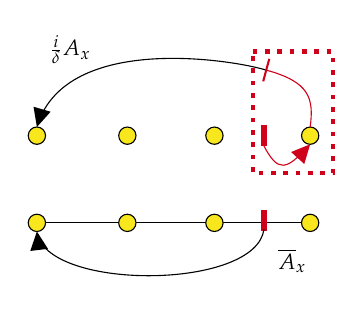
\begin{tikzpicture}[x=0.75pt,y=0.75pt,yscale=-1,xscale=1]
%uncomment if require: \path (0,300); %set diagram left start at 0, and has height of 300

%Shape: Circle [id:dp09874593439383172] 
\draw  [fill={rgb, 255:red, 248; green, 231; blue, 28 }  ,fill opacity=1 ] (3.83,56.58) .. controls (3.83,54.28) and (5.7,52.42) .. (8,52.42) .. controls (10.3,52.42) and (12.17,54.28) .. (12.17,56.58) .. controls (12.17,58.88) and (10.3,60.75) .. (8,60.75) .. controls (5.7,60.75) and (3.83,58.88) .. (3.83,56.58) -- cycle ;
%Shape: Circle [id:dp8464736171323644] 
\draw  [fill={rgb, 255:red, 248; green, 231; blue, 28 }  ,fill opacity=1 ] (89.37,56.58) .. controls (89.37,54.28) and (91.24,52.42) .. (93.54,52.42) .. controls (95.84,52.42) and (97.71,54.28) .. (97.71,56.58) .. controls (97.71,58.88) and (95.84,60.75) .. (93.54,60.75) .. controls (91.24,60.75) and (89.37,58.88) .. (89.37,56.58) -- cycle ;
%Shape: Circle [id:dp8191649989489314] 
\draw  [fill={rgb, 255:red, 248; green, 231; blue, 28 }  ,fill opacity=1 ] (135.5,56.58) .. controls (135.5,54.28) and (137.37,52.42) .. (139.67,52.42) .. controls (141.97,52.42) and (143.83,54.28) .. (143.83,56.58) .. controls (143.83,58.88) and (141.97,60.75) .. (139.67,60.75) .. controls (137.37,60.75) and (135.5,58.88) .. (135.5,56.58) -- cycle ;
%Shape: Circle [id:dp4883813206110459] 
\draw  [fill={rgb, 255:red, 248; green, 231; blue, 28 }  ,fill opacity=1 ] (47.42,56.58) .. controls (47.42,54.28) and (49.28,52.42) .. (51.58,52.42) .. controls (53.88,52.42) and (55.75,54.28) .. (55.75,56.58) .. controls (55.75,58.88) and (53.88,60.75) .. (51.58,60.75) .. controls (49.28,60.75) and (47.42,58.88) .. (47.42,56.58) -- cycle ;
%Straight Lines [id:da4802306696118501] 
\draw    (3.83,98.58) -- (51.58,98.58) -- (143.83,98.58) ;


%Shape: Circle [id:dp8193095728214319] 
\draw  [fill={rgb, 255:red, 248; green, 231; blue, 28 }  ,fill opacity=1 ] (3.83,98.58) .. controls (3.83,96.28) and (5.7,94.42) .. (8,94.42) .. controls (10.3,94.42) and (12.17,96.28) .. (12.17,98.58) .. controls (12.17,100.88) and (10.3,102.75) .. (8,102.75) .. controls (5.7,102.75) and (3.83,100.88) .. (3.83,98.58) -- cycle ;
%Shape: Circle [id:dp28106342849366883] 
\draw  [fill={rgb, 255:red, 248; green, 231; blue, 28 }  ,fill opacity=1 ] (89.37,98.58) .. controls (89.37,96.28) and (91.24,94.42) .. (93.54,94.42) .. controls (95.84,94.42) and (97.71,96.28) .. (97.71,98.58) .. controls (97.71,100.88) and (95.84,102.75) .. (93.54,102.75) .. controls (91.24,102.75) and (89.37,100.88) .. (89.37,98.58) -- cycle ;
%Shape: Circle [id:dp590785861685541] 
\draw  [fill={rgb, 255:red, 248; green, 231; blue, 28 }  ,fill opacity=1 ] (135.5,98.58) .. controls (135.5,96.28) and (137.37,94.42) .. (139.67,94.42) .. controls (141.97,94.42) and (143.83,96.28) .. (143.83,98.58) .. controls (143.83,100.88) and (141.97,102.75) .. (139.67,102.75) .. controls (137.37,102.75) and (135.5,100.88) .. (135.5,98.58) -- cycle ;
%Shape: Circle [id:dp32421153885949106] 
\draw  [fill={rgb, 255:red, 248; green, 231; blue, 28 }  ,fill opacity=1 ] (47.42,98.58) .. controls (47.42,96.28) and (49.28,94.42) .. (51.58,94.42) .. controls (53.88,94.42) and (55.75,96.28) .. (55.75,98.58) .. controls (55.75,100.88) and (53.88,102.75) .. (51.58,102.75) .. controls (49.28,102.75) and (47.42,100.88) .. (47.42,98.58) -- cycle ;
%Straight Lines [id:da7524598861990481] 
\draw [color={rgb, 255:red, 208; green, 2; blue, 27 }  ,draw opacity=1 ][line width=2.25]    (117.42,51.33) -- (117.42,61.58) ;


%Straight Lines [id:da4620382655827757] 
\draw [color={rgb, 255:red, 208; green, 2; blue, 27 }  ,draw opacity=1 ][line width=2.25]    (117.42,92.33) -- (117.42,102.58) ;


%Curve Lines [id:da7042096865740792] 
\draw    (117.42,101.67) .. controls (113.58,130.74) and (15.54,131.32) .. (8.33,104.43) ;
\draw [shift={(8,102.75)}, rotate = 443.02] [fill={rgb, 255:red, 0; green, 0; blue, 0 }  ][line width=0.75]  [draw opacity=0] (8.93,-4.29) -- (0,0) -- (8.93,4.29) -- cycle    ;

%Curve Lines [id:da5752952477375306] 
\draw    (118.5,25) .. controls (102.66,20.05) and (22.95,7.1) .. (8.42,51.07) ;
\draw [shift={(8,52.42)}, rotate = 286.3] [fill={rgb, 255:red, 0; green, 0; blue, 0 }  ][line width=0.75]  [draw opacity=0] (8.93,-4.29) -- (0,0) -- (8.93,4.29) -- cycle    ;

%Curve Lines [id:da38446191206015734] 
\draw [color={rgb, 255:red, 208; green, 2; blue, 27 }  ,draw opacity=1 ]   (117.42,61.58) .. controls (124.22,74.46) and (128.18,73.14) .. (138.36,62.17) ;
\draw [shift={(139.67,60.75)}, rotate = 492.35] [fill={rgb, 255:red, 208; green, 2; blue, 27 }  ,fill opacity=1 ][line width=0.75]  [draw opacity=0] (8.93,-4.29) -- (0,0) -- (8.93,4.29) -- cycle    ;

%Curve Lines [id:da47560590920991563] 
\draw [color={rgb, 255:red, 208; green, 2; blue, 27 }  ,draw opacity=1 ]   (139.67,52.42) .. controls (141.5,38.67) and (139.5,30.67) .. (118.5,25) ;
\draw [shift={(118.5,25)}, rotate = 375.1] [color={rgb, 255:red, 208; green, 2; blue, 27 }  ,draw opacity=1 ][line width=0.75]    (0,5.59) -- (0,-5.59)   ;

%Shape: Rectangle [id:dp6553128643132535] 
\draw  [color={rgb, 255:red, 208; green, 2; blue, 27 }  ,draw opacity=1 ][dash pattern={on 1.69pt off 2.76pt}][line width=1.5]  (112,16) -- (150.5,16) -- (150.5,74.67) -- (112,74.67) -- cycle ;

% Text Node
\draw (24,15) node [scale=0.8]  {$\frac{i}{\delta } A_{x}$};
% Text Node
\draw (131,117) node [scale=0.8]  {$\overline{A}_{x}$};


\end{tikzpicture}

Généralisation
\begin{align*} 
	\Ax*{\termxn} &\stackrel{DUD}= \frac{i}{\delta} \Ax{\termxn} &
	\Ax*{x:\angln} &\stackrel{DUD}= \frac{i}{\delta} \Ax{\termxn} + \Ax{x:\nthtop{1}{\angln}} 
\end{align*}

Cas de croissance
\begin{align*} 
\twoletsymb{{\color{purple}\bar{I}}}{\bar{A}}_{x}
	&\stackrel{DUD}= \frac{i}{\delta} \left[\twoletsymb{I}{A}_x {\color{purple} - \bigg( \frac{1}{d} - \frac{1}{\delta} \bigg) \Ax{x}} \right] \\
\twoletsymb{I^{{\color{orange}(m)}}}{A}_{x}^{(m)}
	&\stackrel{DUD}= \frac{i}{i^{(m)}} \left[\twoletsymb{I}{A}_x {\color{orange} - \bigg( \frac{1}{d} - \frac{1}{d^{(m)}} \bigg) \Ax{x}} \right] \\
\end{align*}

Généralisation avec multiple de la force d'intérêt
\begin{align*} 
	\prescript{j}{}{\Ax*{x}} &\stackrel{DUD}= \frac{e^{j\delta} - 1}{j \delta} \prescript{j}{}{\Ax{x}} &
	 \prescript{j}{}{\Ax{x}}^{(m)} &\stackrel{DUD}=  \frac{e^{j\delta} - 1}{m(e^{\frac{j\delta}{m}} - 1)} \prescript{j}{}{\Ax{x}} 
\end{align*}

\paragraph{Approximations}

\begin{align*} 
	\Ax*{x} &\approx (1 + i)^{\frac{1}{2}} \Ax{x}	&
	\Ax{x}^{(m)} &\approx (1 + i)^{\frac{m - 1}{2m}} \Ax{x}
\end{align*}

\begin{align*} 
	\twoletsymb{D}{\bar{A}}_{\nthtop{1}{x}:\angln} 
		&\approx (1 + i)^{\frac{1}{2}} \twoletsymb{D}{A}_{\nthtop{1}{x}:\angln}		&
	\Ax*{x:\angln} 
		&\approx (1 + i)^{\frac{1}{2}} \Ax{\termxn} + \Ax{x:\nthtop{1}{\angln}}  \\
\end{align*}

\begin{align*}
	\twoletsymb{\bar{D}}{\bar{A}}_{\nthtop{1}{x}:\angln} 
		&\approx (1 + i)^{\frac{1}{2}} 
		\left[
			\twoletsymb{D}{A}_{\nthtop{1}{x}:\angln}	-
			\frac{1}{2}	\Ax{\nthtop{1}{x}:\angln}
		\right] \\
	\twoletsymb{I_{\angln}^{(m)}}{\bar{A}}_{x} 
		&\approx (1 + i)^{\frac{1}{2}} 
		\left[
			\twoletsymb{I_{\angln}}{A}_{x}	-
			\frac{m - 1}{2m}	\Ax{\nthtop{1}{x}:\angln}
		\right]
\end{align*}

\section{Contrats de rente}
\paragraph{Rente viagère} On verse une rente à l'assuré jusqu'à son décès. 
\begin{align*}
Y	&  = \ax*{\angl{T_{x}}} = \frac{1-v^{T_x}}{\delta} = \frac{1 -\overline{Z}_x}{\delta} \\
\ax*{x} & = \int_{0}^{\infty}  \ax*{\angl{T_{x}}}  \px[t]{x} \mu_{x+t} dt \\
	& = \int_{0}^{\infty} v^t \px[t]{x} dt \\
	& = \frac{1 - \Ax*{x}}{\delta} \\
\variance{Y}	& = \variance{\frac{1- v^{T_x}}{\delta}} =  \frac{\Ax*[][2]{x} - \Ax*{x}^2}{\delta^2} \\
\end{align*}

\paragraph{Rente temporaire $n$ années} Ce contrat de rentes prévoit payer une rente à l'assuré s'il est en vie, au maximum $n$ années.
\begin{align*}
Y & = \begin{cases}
\ax*{\angl{T_x}}	& , T_x < n \\
\ax*{\angln}			& , T_x \geq n \\
\end{cases} = \frac{1  - \overline{Z}_{x:\angln}}{\delta} \\
\ax*{x:\angln}	& = \int_{0}^{n} \ax*{\angl{t}} \  \px[t]{x} \  \mu_{x+t} dt \\
	& = \int_{0}^{n} v^t \px[t]{x} dt \\
	& = \frac{1 - \Ax*{x:\angln}}{\delta} \\
\variance{Y}	& = \frac{\Ax*[][2]{x:\angln} - \Ax*{x:\angln}^2}{\delta^2} \\	
 \end{align*}

\paragraph{Rente viagère différée $m$ années} C'est un contrat de rente viagère, qui débute dans $m$ années (si $(x)$ est en vie).
\begin{align*}
Y & = \begin{cases}
0											& T_x	 < 	 m	\\
v^m \ax*{\angl{T_x - m}}	& T_x 	\geq m	\\
\end{cases} = \frac{\overline{Z}_{20:\itop{\angl{10}}} - \prescript{}{m|}{\overline{Z}}_{20}}{\delta} \\ 
\ax*[m|]{x}	& = \int_{m}^{\infty} \ax*{t-m} \px[t]{x} \mu_{x+t} dt \\
	& = \Ex[m]{x} \ax*{x+m} \\
	& = \ax*{x} - \ax*{x:\angl{m}} \\
\end{align*}

\paragraph{Rente garantie (certaine) $n$ années} Le contrat prévoit une rente minimale de $n$ années, pouvant se prolonger jusqu'au décès de l'assuré.
\begin{align*}
Y & = \begin{cases}
\ax*{\angln}	& = T_x < n \\
\ax*{\angl{T_x}}	& = T_x \geq n \\
\end{cases} = \overline{Y}_{x:\angln} + \prescript{}{n|}{Y}_x \\
\ax*{\joint{x:\angln}}	& =\ax*{\angln} \cdot \qx[n]{x} + \int_{n}^{\infty} \ax*{\angl{t}} \px[t]{x} \mu_{x+t} dt \\
	& = \ax*{\angln} + \ax*[n|]{x} \\
\end{align*}

\section{Primes nivelées}
\subsection{Notation et définitions}
On définit $L$ comme la perte à l'émission d'un contrat pour l'assureur. Dans ce chapitre, le paiement de la PUN s'étalle sur une période de temps, et est conditionnel  à la survie de l'assuré. Dans le cas d'une assurance-vie,
\[L = Z - Y\]
où $Z$ est la valeur présente actuarielle est prestations à payer et $Y$ la valeur présente actuarielle des primes à recevoir. De même, pour les rentes,
\[L = Y_1 - Y_2\]
où $Y_1$ représente la valeur présente actuarielle des prestations de rente à payer et $Y_2$ la valeur présente actuarielle des primes à recevoir. \\

On définit la prime nette nivellée $\pi$ selon 3 principes. 

\subsection{Principe d'équivalence (PE)}
Sous le principe d'équivalence, $\pi^{PE}$ est la solution de
\begin{align*}
\esp{L}	& = 0 \\
\esp{Z} - \esp{Y}	& = 0 \\
\esp{Z} & = \esp{Y} \\
\end{align*}


\subsection{Principe de la perte maximale probable (PPMP)}
Sous le Principe de la perte maximale probable, $\pi^{PPMP}$ est la solution de
\begin{align*}
\prob{L < \lambda} \geq \alpha
\end{align*}
Pour résoudre, on va plutôt exprimer $\prob{L < \lambda} \leftrightarrow \px[t^*]{x}$ pour solutionner $\pi^{PPMP}$.


\subsection{Principe du portefeuille (PP)}
Similaire au PPMP, en terme de \emph{portefeuille} : $\pi^{PP}$ est la solution de
\begin{align*}
\prob{\frac{L_1 + ... + L_n}{n} < \lambda} &  \geq \alpha \\
\prob{L_1 + ... + L_n < n \lambda} & \geq \alpha \\
\end{align*}
On passe par le Théorème central limite (TCL) pour évaluer cette expression. Ainsi,
\begin{gather*}
\prob{\frac{L_1 + ... + L_n - \esp{L_1 + ... + L_n}}{\sqrt{\variance{L_1 + ... + L_n}}} < \frac{n \lambda - \esp{L_1 + ... + L_n}}{\sqrt{n \variance{L}}}  }  \geq \alpha \\
\shortintertext{Puisque les pertes à l'émission sont \emph{iid,}} \\
\prob{Z < \frac{n \lambda - n \esp{L}}{\sqrt{n \variance{L}}}}  \geq \alpha \\
\shortintertext{Par le TCL,} \\
\Phi \left( \frac{n \lambda - n \esp{L}}{\sqrt{n \variance{L}}} \right)  \geq \alpha \\
\end{gather*}
Où $Z \sim N(0,1)$ et $\Phi$ la fonction de répartition de $Z$. Le défi se trouve dans le calcul de $\variance{L}$, où
\begin{align*}
\variance{L}	& = \variance{Z - Y} \\
& = \variance{Z} + \variance{Y} - 2 \  \covar{Z, Y} \\
& = \variance{Z}  + \variance{Y} - 2 \left( \esp{ZY} - \esp{Z} \esp{Y} \right) \\
\end{align*}

\subsection{Retour de primes}
\begin{itemize}
\item Certains contrats (surtout rentes différée) vont prévoir un remboursement partiel ($\alpha$) ou total des cotisations (accumulées au taux $j < i$)\footnote{Le taux $i$ est le taux préférentiel de l'assureur, tandis que le taux $j$ est le taux offert à l'assuré pour l'accumulation de ses cotisations dans sa clause de retour de primes.} en cas de décès de l'assuré pendant la période différée.
\item On introduit la v.a. $W$, qui représente la valeur présente actuarielle d'un retour de prime, telle que
\begin{align*}
W = 
\begin{cases}
\alpha \pi v_i^{K_x + 1} \sx**{\angl{K_x + 1}j} & K_x = 0, 1, ..., n-1 \\
0	& K_x = n, n+1, ... \\
\end{cases}
\end{align*}
Alors,
\[L = Y_1 - Y_2 + W\]
\item Aussi, on trouve que
\[\esp{W} = \sum_{k=0}^{n - 1} \alpha \pi v_i^{k+1} \sx**{\angl{k+1} j} \qx[k|]{x} = \alpha \pi \psi\]
\end{itemize}

\subsection{Primes brutes}
\begin{itemize}
\item Pour tenir compte des dépenses de l'assureur, on calcule la prime \emph{brute} $G$, qui considère la valeur actualisée des dépenses de l'assureur $D$ dans le calcul de la perte à l'émission.
\item Alors, on a
\[L = Z + D - Y\]
avec $Y$ qui est fonction de $G$ (la prime brute), et non $\pi$.
\item Il y a 3 types de dépenses : 
\begin{enumerate}[label=\Roman*)]
	\item Dépenses initiales ;
	\begin{enumerate}[label=\textbullet]
		\item À l'émission du contrat ; 
		\item Commission des ventes (\% de $G$ ou du montant d'assurance $M$) ;
		\item Coût des employés qui saisissent les informations dans le système ;
		\item Impression et envoi par courrier de la police.
		\item ...
	\end{enumerate}
	\item Dépenses de renouvellement ;
	\begin{enumerate}[label=\textbullet]
		\item Commission de renouvellement (\% de $G$ ou du montant d'assurance $M$), si $G$ est payée (i.e. conditionnel à la survie de l'assuré).
	\end{enumerate}
	\item Dépenses de fin de contrat.
	\begin{enumerate}[label=\textbullet]
		\item Saisie informatique et frais de fermeture de dossier ;
		\item Émission du chèque de prestations ;
		\item Enquête (dans certains cas).
	\end{enumerate}
\end{enumerate}
\end{itemize}











\end{multicols*}
%% -----------------------------
%% Fin du document
%% -----------------------------
\end{document}
